% Kandidate prosimo, da nam posredujejo predloge za izbolj''save tega vzorca 
% na elektronski naslov Fizikalne knji''znice: fiz.knjiz@fmf.uni-lj.si.
%-----------------------------------------------------------------------------------------
%        METAPODATKI
%-----------------------------------------------------------------------------------------

\begin{filecontents*}{\jobname.xmpdata}
\Title{Quenchi čez fazni prehod topološkega izolatorja z neredom}			                %%% vnesite svoj naslov magistrskega dela
\Author{mag. Andrej Kolar - Požun}					                %%% vnesite svoje ime in priimek
\Keywords{magisterij\sep navodila\sep ključne besede} %%% vnesite svoje ključne besede
\Subject{Fizika}	
\end{filecontents*}

%-----------------------------------------------------------------------------------------

\documentclass[longbibliography,slovene,a4paper,12pt]{book}

\usepackage[slovene]{babel}    
\usepackage[utf8]{inputenc}
\usepackage{amsfonts}
\usepackage[T1]{fontenc}
\usepackage[pdftex]{graphicx}
\usepackage{fancyhdr}
\usepackage[sort, numbers]{natbib}
\usepackage{acro}
\usepackage[nottoc,numbib]{tocbibind}
\usepackage{amsmath}
\usepackage{graphicx}
\usepackage{amsthm}
\usepackage{subcaption}
\usepackage{amssymb}
\usepackage{caption}
\usepackage{float}
\usepackage{romannum}
\usepackage{physics}
\usepackage{multicol}
\newtheorem*{theorem*}{Birkhoff-Kichinov izrek}
  
%---------------------------------------------------------------------------------------------
%        PDF/A
%---------------------------------------------------------------------------------------------

\usepackage{xmpincl}
\usepackage[a-1b]{pdfx}       

%----------------------------------------------------------------------------------------------

\usepackage{filecontents}
\usepackage{hyperref}
\usepackage{url}
\usepackage[a4paper,inner=3.5cm,outer=2.5cm,top=2.5cm,bottom=2.5cm,pdftex]{geometry}
\usepackage[titletoc,title]{appendix}
\usepackage{epstopdf}
\usepackage{makeidx}
\pagestyle{fancy}
\setlength{\headheight}{15pt}
\usepackage{enumitem}
\usepackage{underscore}
\usepackage{tocloft}
\renewcommand{\cftpartleader}{\cftdotfill{\cftdotsep}} 
\renewcommand{\cftchapleader}{\cftdotfill{\cftdotsep}} 

\makeindex

\def\epsfg#1#2{\epsfig{file=#1.eps,width=#2}}
\def\legendamp#1#2{\vbox{\hsize=#1\caption{\small #2}}}

\setcounter{topnumber}{4}
\setcounter{bottomnumber}{4}
\setcounter{totalnumber}{5}
\renewcommand{\topfraction}{0.99}
\renewcommand{\bottomfraction}{0.99}
\renewcommand{\textfraction}{0.0}
\setlength{\tabcolsep}{10pt}
\renewcommand{\arraystretch}{1.5}

\def\bi#1{\hbox{\boldmath{$#1$}}}
\let\oldvec\vec
\def\vec#1{\mbox{\boldmath$#1$}}
\def\pol{{\textstyle{1\over2}}}
\def\svec#1{\mbox{{\scriptsize \boldmath$#1$}}}


%----------------------------------------------------------------------------------------
%    SUMNIKI
%----------------------------------------------------------------------------------------
%% Za pisanje sumnikov imamo tri moznosti:
%%   --- vnasamo jih neposredno v kodnem sistemu UTF-8 
%%   --- pisemo jih z latexovim ukazom, ki je namenjen natanko temu,
%%       in sicer kot \v{c}, \v{s}, \v{z}, \v{C}, \v{S}, v{\Z} ali
%%       malo manj pregledno kot \v c, \v s, \v z, \v C, \v S, \v Z,
%%   --- pisemo jih kot "c, "s, "z, "C, "S, "Z), vendar tedaj potrebujemo
%%       spodaj zapisani macro, ki znaku " pripise vlogo `izdelave' sumnika:
\catcode`\"=\active\def"#1{\v{#1}}
%%       torej \v{S}krjan\v{c}ek == \v Skrjan\v cek == "Skrjan"cek
%% Pozor: narekovaj potem ne smemo vec pisati kot " ampak kot `` in '',
%%       torej: "Skrjan"cek je "civkal ``"ci-"ci-"ci''.
%
%------------------------------------------------------------------------------------------

\begin{document}

%--------------------------------------------------------------------------------------
%       NASLOVNA STRAN
%-----------------------------------------------------------------------------------

\pagestyle{empty}
\begin{center}

{\large UNIVERZA V LJUBLJANI\\
FAKULTETA ZA MATEMATIKO IN FIZIKO\\
ODDELEK ZA FIZIKO\\
MATEMATIČNA FIZIKA\\}


\vspace{4cm}


{\Large Andrej Kolar - Požun\\}

\vspace{10mm}

{\bf \Large QUENCHI ČEZ FAZNI PREHOD TOPOLOŠKEGA IZOLATORJA Z NEREDOM}\\
\vspace{5mm}
{\large Magistrsko delo}\\




\vfill



{\large MENTOR: dr. Tomaž Rejec\\
SOMENTORICA: mag. Lara Ulčakar\\


\vspace{2cm}
Ljubljana, 2020}

\end{center}

%--------------------------------------------------------------------------
%        ZAHVALA (NEOBVEZNO)
%--------------------------------------------------------------------------

\cleardoublepage
\mbox{}
\vfill
{\Large \bf Zahvala}
\vspace{1cm}\\
hvala

%------------------------------------------------------------------------
%         IZVLECEK
%-----------------------------------------------------------------------

\cleardoublepage
\begin{center}
{\bf Naslov v slovenskem jeziku}\\[3mm]
{\sc  Izvle"cek}
\end{center}
\vspace{10mm}
V delu obravnavamo model eno dimenzionalnega topološkega izolatorja z neredom. Pokažemo, da lahko med topološkima fazama prehajamo tudi z višanjem jakosti nereda in pokažemo nenavadne lastnosti te točke faznega prehoda. V nadaljevanju izvajamo preklop lastnega stanja v netrivialni topološki fazi čez fazni prehod z višanjem jakosti nereda v trivialno fazo. Pri prehodu se pojavijo eksitacije, katerih število je odvisno od hitrosti in intervala preklopa. Pokažemo, da je odvisnost števila eksitacij od hitrosti potenčna z nenavadnimi potencami. Nadalje se poglobimo v podrobnosti posameznih eksitacij, kjer opazimo, da eno preklopljena stanje praviloma preide v le dve stanji v prevodnem pasu. \\[10mm]
{\bf Klju"cne besede:}\\[3mm]

\cleardoublepage

 \foreignlanguage{english}{  %  angleski delilni vzorci
\begin{center}
{\bf Naslov v angleškem jeziku}\\[3mm]
{\sc  Abstract}
\end{center}
\vspace{10mm}
Kratek izvleček v angleškem jeziku, do 300 besed.\\[10mm]
{\bf Keywords:}\\[3mm]
}

%------------------------------------------------------------------------
%        KAZALO
%----------------------------------------------------------------------

\cleardoublepage
\tableofcontents

%------------------------------------------------------------------------
%       OSREDNJI DEL
%-------------------------------------------------------------------------

\pagestyle{fancy}
\fancyhead[CE,RE]{}
\fancyhead[LO,CO]{}
\fancyhead[LE]{\textbf{\nouppercase{\leftmark}}}
\fancyhead[RO]{\textbf{\nouppercase{\rightmark}}}

%\input{Uvod}

\chapter{Uvod}
\label{chUv}
Že dolgo časa je znano, da lahko večino fizikalnih sistemov v fiziki trdne snovi klasificiramo med prevodnike in izolatorje, odvisno od obstoja energijske reže v spektru Hamiltonjana. V zadnjih desetletjih pa so raziskovalno popularni posebni tipi izolatorjev - topološki izolatorji. Te lahko nadalje klasificiramo v različne topološke faze, katerih ureditveni parameter je celoštevilska topološka invarianta. Ti materiali so zanimivi, ker so topološke invariante invariantne na zvezne transformacije, kar pomeni, da so topološke faze robustne na infinitezimalno majhne petrurbacije - če želimo iti v drugo fazo, moramo narediti nekaj nezveznega ali pa spremeniti enega izmed glavnih lastnosti modela, na primer zapreti energijsko režo ali zlomiti eno izmed simetrij modela. Poleg tega je pri topoloških izolatorjih, za razliko od navadnih materialov, rob materiala pomemben tudi v termodinamski limiti. Kljub izolatorski fazi v notranjosti materiala imamo namreč lahko na robu prisotna prevodna stanja, katerih število je povezano s topološko invarianto v notranjosti. Ta pojav je znan kot notranjost-rob korepondenca. Zaradi robustnosti topološke invariante so tudi ta robna stanja robustna, kar pomeni, da topološki izolator lahko predstavlja dober prevodnik, ki je robusten na nečistoče v materialu. Iz notranjost-rob korespondence pa izhaja še ena tehnološka aplikacija topoloških izolatorjev: Če imamo na voljo način za zlom simetrije, ki povzroči prehod med fazami, lahko na roke spreminjamo topološko invarianto sistema in s tem število prevodnih stanj na robu, kar je potrebna lastnost za izgradnjo kvantnega tranzistorja, ki bi se lahko uporabljal v kvantnih računalnikih. MOGOČE BI ZA MOTIVACIJO LAHKO POVEDAL DA SO TUDI NASPLOH TOPOLOŠKE FAZE ENA GLAVNIH IDEJ ZA KUBITE ZA KVANTNE RAČUNALNIKE

V tem delu se bomo posvetili eno-dimenzionalnem topološkem izolatorju z nečistočami. Povedali smo že, da so topološke faze robustne na nečistoče v materialu, vendar to velja le, ko te niso premočne. Ko so premočne sistem preide v trivialno topološko fazo. NE VEM ČE BI POVEDAL TU ŠE KAJ O TEJ TOČKI, NPR DELOKALIZACIJA
V magisteriju bomo izvajali preklop, torej, časovni razvoj stanja pri časovno odvisnem Hamiltonjanu, čez ta fazni prehod z večanjem jakosti nereda. Zaradi končne hitrosti preklopa se pri tem v valenčnem času pojavijo eksitacije. Glavni cilj dela je pokazati potenčno skaliranje števila eksitacij v odvisnosti od hitrosti preklopa. Motivacija za iskanje takšnega skaliranje je Kibble-zurekov mehanizem \cite{kibble}, ki velja za preklope med navadnimi (torej ne topološkimi) fazami in predvideva prav takšno skaliranje (JE TO RES? GOVORIMO O TOPOLOŠKIH DEFEKTIH AMPAK PRI KIBBLE ZUREKU VIDIM VES CAS OMENJEN ZLOM SIMETRIJE, KI GA PRI TOPOLOSKIH FAZAH NIMAMO A NE).
\chapter{Topološki izolatorji}
\label{chMa}

\section{SSH model}
Najpreprostejši model topološkega izolatorja je Su-Schrieffer-Heegerjev (SSH) model, ki obravnava eno-dimenzionalno Bravaisovo rešetko (verigo) z bazo, kjer je osnovna celica sestavljena iz dveh mest, ki ju označimo s črkama A in B. V modelu, podobno kot v tesni vezi, obravnavamo elektron, ki skače med najbližjimi sosedi na verigi. Kot je razvidno na Sliki \ref{fig:chain}, je skakanje med mestama v isti osnovni celici določeno s sklopitvenim parameterom $v$, medtem ko je skakanje med sosednjimi mesti iz različnih osnovnih celic določeno z (v splošnem različnim) parameterom $w$.
\begin{figure}[H]
\centering
\begin{subfigure}{.9\textwidth}
\includegraphics[width=\linewidth]{Figures/MySSHChain.pdf}
\end{subfigure}
\caption{Atomska veriga, ki ustreza SSH modelu. Svetlo in temno sivi krogi ustrezajo mestom tipa A in B. Osnovna celica je označena z modro, črtkano črto. Veriga na sliki je sestavljena iz petih osnovnih celic. Skakanje v osnovni celici je določeno s parametrom $v$ in s črto z pikicami, medtem ko je prehajanje med osnovnimi celicami (parameter $w$) označeno s črto s črtkami.}
\label{fig:chain}
\end{figure}
Če prevedemo zgornje napisano v Hamiltonski opis, dobimo SSH-jev Hamiltonjan \cite{SSH}:
\begin{equation}
\hat{H} = v \sum_{m=1}^{\frac{N}{2}} \left( |m, B \rangle \langle m, A | + \textup{h. c.} \right) + w \sum_{m=1}^{\frac{N}{2}-1} \left( | m+1, A \rangle \langle m, B | + \textup{h. c.} \right),
\end{equation}
kjer $|m , \alpha \rangle = |m \rangle \otimes | \alpha \rangle$, z $m=1,.., \frac{N}{2}$ and $\alpha \in \{A,B\}$ označuje stanje elektrona, ki je lokalizirano na podmreži $\alpha$ v $m$-ti osnovni celici. Število vseh mest v verigi je $N$, kar pomeni, da je osnovnih celic $\frac{N}{2}$.  Analogno razdelimo tudi naš Hamiltonjan na del, ki deluje na zunanjo prostorsko stopnjo $|m \rangle$ in na del, ki deluje na notranjo prostorsko stopnjo $| \alpha \rangle$:
\begin{equation}
\hat{H} = v \sum_{m=1}^{\frac{N}{2}} |m \rangle \langle m| \otimes \hat{\sigma}_x + w \sum_{m=1}^{\frac{N}{2}-1} \left( | m+1\rangle \langle m | \otimes \frac{\hat{\sigma}_x + i \hat{\sigma}_y}{2} + \textup{h. c.} \right).
\end{equation}
\newpage
\subsection{Fizika translacijsko invariantnega sistema}
Za trenutek pozabimo na rob verige in se osredotočimo na njeno notranjost. Zanima nas torej dolg, sredinski del verige, ki prostorsko prevlada v termodinamski limiti $N \to \infty$. Kot vemo, \cite{ashcroft} fizika v notranjosti materiala ni odvisna od dogajanja na robu, torej lahko za njeno obravnavo izberemo najpreprostejše robne pogoje - periodične robne pogoje. Takšni robni pogoji ustrezajo translacijsko invariantnem sistemu, za kar uvedimo oznako TIS. Hamiltonjan, ki opisuje to fiziko $\hat{H}_{\textup{TIS}}$ lahko torej dobimo iz prejšnjega Hamiltonjana, če vanj preprosto dodamo člen $w\ | N/2, B \rangle \langle 1, A|$  (in seveda njegovo hermitsko konjugiranko), ki opiše interakcijo med prvo in zadnjo osnovno celico prvotne verige in jo s tem transformira v periodično verigo.
Iščemo $N$ lastnih stanj Hamiltonjana $|\Psi_n (k) \rangle$ z energijami $E_n(k)$:
\begin{equation}
\hat{H}_{\textup{TIS}} | \Psi_n (k) \rangle = E_n(k) | \Psi_n(k) \rangle.
\end{equation} 
V zgornji enačbi smo že zapisali energije in stanja kot funkcije Blochovega vektorja $k$, saj vemo, da za translacijsko invariantne sisteme veljla Blochov teorem \cite{ashcroft} in lahko napišemo lastna stanja v naslednji obliki:
\begin{equation}
| \Psi_n (k) \rangle = | k \rangle \otimes | u_n (k) \rangle.
\end{equation}
V zgornji enačbi smo vpeljali Blochovo funkcijo $|k\rangle$:
\begin{equation}
|k \rangle = \frac{1}{\sqrt{N/2}} \sum_{m=1}^{\frac{N}{2}} e^{imk} |m \rangle,
\end{equation}
kjer $k$ zavzame $\frac{N}{2}$ različnih vrednosti v prvi Brillouinovi coni.
Zdaj lahko definiramo še Hamiltonjan v recipročnem prostoru $\hat{H}(k) = \langle k | \hat{H}_{\textup{TIS}} | k \rangle$, ki deluje na notranjo prostorsko stopnjo:
\begin{equation}
\hat{H}(k) | u_n(k) \rangle = E_n(k) | u_n(k) \rangle.
\end{equation}
Če razvijemo notranji del valovne funkcije po podmrežni bazi $|u_n(k) \rangle = a_n(k) |A \rangle + b_n(k) | B \rangle$,
$\hat{H}(k)$ postane 2x2 (hermitska) matrika in se torej lahko zapiše kot linearna kombinacija Paulijevih matrik in identitete:
\begin{equation}
H(k) = d_0 (k) \mathbb{I}+ d_x(k) \sigma_x + d_y (k) \sigma_y + d_z(k) \sigma_z.
\end{equation}
Iz koeficientov razvoja tvorimo vektor $\vec{d}(k) = (d_x,d_y,d_z)(k)$ iz katerega bomo dobili topološke lastnosti modela \cite{madzar}. Izkaže se, da je za SSH model $d_z(k)$ enak nič. Ko višamo $k$ od $0$ proti $2 \pi$, vektor $\vec{d}(k)$ torej oriše krivuljo v dvo-dimenzionalni $(d_x,d_y)$ ravnini. Zaradi periodičnosti Brillouinove cone mora ta krivulja biti zanka, katero lahko topološko klasificiramo s celoštevilskim parametrom: ovojnim številom okoli izhodišča $\nu$ \cite{hatcher}. Kot bo jasneje na primerih, nam ovojno število pove kolikokrat se orientirana zanka "ovije" okoli izhodišča.
Konkretno lahko, z eksplicitno konstrukcijo Hamiltonjana v recipročnem prostoru dobimo vektor:
\begin{equation}
\vec{d}(k) = (v + w \cos k, w \sin k, 0).
\end{equation}
Zanke, ki ustrezajo različnim izbiram parametrov $v, w$ lahko vidimo v drugi vrstici na Sliki \ref{fig:examples}. Za $w < v$ imamo $\nu = 0$, medtem ko $w > v$ da $\nu=1$. Primer, ko velja $w=v$ je poseben, saj v tem primeru zanka $\vec{d}(k)$ gre skozi izhodišče, kar pomeni, da je ovojno število okoli izhodišča nedefinirano.
V prvi vrstici na Sliki \ref{fig:examples} je prikazana disperzijska relacija za vsak obravnavam primer. Dobimo jo z diagonalizacijo Hamiltonjana v recipročnem prostoru kar da:
\begin{equation}
E(k) = \pm \sqrt{v^2 + w^2 + 2 w v \cos k}
\end{equation}
Vidimo lahko, da je za primere $v \neq w$ prisotna končna energijska reža med prevodnim in valenčnim pasom kar po definiciji ustreza izolatorju. Pri posebni točki $v=w$, kjer je ovojno število nedefinirano se energijska reža zapre in sistem preide v prevodno stanje. Opravka imamo torej z dvema možnima izolatorskima fazama, ki se razlikujeta po ureditvenem parameteru $\nu$. Primeru $\nu=0$ bomo rekli trivialna faza, medtem ko primer $\nu=1$ ustreza topološki fazi. Ovojno število je topološka invarianta v naslednjem smislu: Ohranjajo ga zvezne deformacije (homotopije) zank, ki se izognejo izhodišču. Zvezen prehod med različnima izolatorskima fazama je torej možen le s prehodom skozi prevodno stanje (kar geometrijsko pomeni, da med homotopijo zanka preide skozi izhodišče). K tej lastnosti modela se bomo kasneje vrnili v splošnejšem smislu.
\begin{figure}[H]
\centering
\begin{subfigure}{.9\textwidth}
\includegraphics[width=\linewidth]{Figures/GapAndTopology.pdf}
\end{subfigure}
\caption{V prvi vrstici je prikazana disprezijska relacija za različne kombinacije parametrov $v$ in $w$. V drugi vrstici so narisane zanke $\vec{d}(k)$ v $(d_x , d_y)$ ravnini. Prva stolpca ustrezata $\nu = 0$, zadnja ustrezata $\nu = 1$, medtem ko gre v sredinskem zanka skozi izhodišče in je $\nu$ nedefiniran. Vir Slike: \cite{madzar}}
\label{fig:examples}
\end{figure}

Za konec omenimo še, da za ovojno število obstaja eksplicitna formula.
Ker se zanka izogne izhodišču, jo lahko projeciramo na enotsko kroznico z normiranjem vektorja $\vec{d}(k)$:
\begin{equation}
\widehat{r}(k) = \frac{\vec{d}(k)}{|\vec{d}(k)|}.
\end{equation}
Zanima nas celotna sprememba polarnega kota $\Delta \varphi$ tega vektorja, ko gre $k$ od $0$ do $2 \pi$. Ker imamo opravka z zanko, mora ta sprememba biti celoštevilki večkratnik $2 \pi$ oziroma po definiciji ovojnega števila $\Delta \varphi = \nu 2 \pi$, torej velja
\begin{equation}
\nu = \frac{1}{2  \pi} \Delta \varphi = \frac{1}{2 \pi} \int_{k=0}^{k=2 \pi} \textup{d}\varphi(k)
\end{equation}
Izraz za polarni kot in njegov diferencial poznamo:
\begin{align}
&\varphi(k) = \arctan (\widehat{r}_y(k) / \widehat{r}_x(k)) \\
&\textup{d} \varphi(k) = - \widehat{r}_y(k) \textup{d} \widehat{r}_x(k) +  \widehat{r}_x(k) \textup{d} \widehat{r}_y(k) = \left( \widehat{r}(k) \times \textup{d} \widehat{r}(k) \right)_z,
\end{align}
Tako dobimo končno formulo za ovojno število, izraženo z zanko $\widehat{r}(k)$:
\begin{equation}
\nu = \frac{1}{2 \pi} \int_{k=0}^{k=2 \pi}  \left( \widehat{r}(k) \times \textup{d} \widehat{r}(k) \right)_z = \frac{1}{2 \pi} \int_0^{2 \pi} \left ( \widehat{r}(k) \times \frac{\textup{d}}{\textup{d} k} \widehat{r}(k) \right)_z \textup{d}k
\end{equation}
Ovojno število lahko izrazimo neposredno s pomočjo matrike Hamiltonjana v impulznem prostoru, če se spomnemo, da je naddiagonalna komponenta enaka
$h(k) = d_x (k) - i d_y(k)$. Če izračunamo kompleksen logaritem te komponente:
\begin{equation}
\ln h(k) = \ln (|h(k)|) + i \arg h(k) = \ln(d_x^2(k) + d_y^2(k)) + i \arctan (d_y(k) / d_x(k)),
\end{equation}
opazimo, da lahko zgornjo formulo za ovojno število napišemo tudi kot:
\begin{equation}
\nu = \frac{1}{2 \pi i} \int_{- \pi}^\pi \frac{\textup{d}  \ln h(k) }{\textup{d} k}\textup{d}k.
\end{equation}
\subsection{Robna stanja}
V prejšnjem poglavju smo raziskali fiziko v notranjosti materiala, zdaj pa se osredotočimo na robna stanja. 

Začnimo s preprostim primerom. Za trenutek obravnavajmo spet verigo brez robnih pogojev in poglejmo dva limitna primera - tako imenovani popolnoma dimerizirani limiti, kjer enega od sklopitvenih parametrov $v$ ali $w$ postavimo na nič. Posledično veriga razpade na nepovezane komponente imenovane "dimeri", kot je vidno na Sliki \ref{fig:dimerized}.

\begin{figure}[H]
\centering
\begin{subfigure}{.9\textwidth}
\includegraphics[width=\linewidth]{Figures/MyDimerized1.pdf}
\end{subfigure}
\begin{subfigure}{.9\textwidth}
\includegraphics[width=\linewidth]{Figures/MyDimerized2.pdf}
\end{subfigure}
\caption{Različni popolnoma dimerizirani limiti SSH verige. Zgornja slika prikazuje primer, ko je $w=0$, spodnja pa, ko je $v=0$. Dimeri, ki nastanejo so obkroženi z rdečo črto. V primeru, ko velja $w=0$, je vsako mesto del nekega dimera, medtem ko na spodnji sliki dobro vidimo mesti, ki nista del dimerov in ustrezata robnim stanjem.}
\label{fig:dimerized}
\end{figure}

V prvem primeru imamo $w=0, v > 0$, kar ustreza trivialni fazi ($\nu=0$). $N$ lastnih funkcij in njihove energije so:
\begin{equation}
H ( |m, A \rangle \pm | m , B \rangle) = \pm v( |m, A \rangle \pm | m, B \rangle ).
\end{equation}
Stanja elektronov so lokalizirana na posameznih dimerih, ki sovpadajo z osnovnimi celicami.
V drugem primeru imamo $v=0, w>0$, kar ustreza topološki fazi ($\nu = 1$):
\begin{equation}
H ( |m, B \rangle \pm | m + 1 , A \rangle) = \pm w( |m, B \rangle \pm | m+1,A \rangle ).
\end{equation}
Spet je elektron lokaliziran na dimerih, ki pa zdaj ne sovpadajo več z osnovnimi celicami, ampak vsebujejo mesti s sosednjih osnovnih celic.
V obeh primerih je energija enaka $\pm v$ ali $\pm w$, torej so energijski pasovi ravni, kar pomeni, da je grupna hitrost elektronov nič \cite{ashcroft}, kar je smiselno, saj so lokalizirani na posameznih dimerih.

V trivialni fazi nam da zgornja formula vseh $N$ stanj.  Po drugi strani pa da za topološko fazo zgornja formula le $N-2$ stanj. Izkaže se, da sta v topološki fazi izolirani mesti na robu, vidni na Sliki \ref{fig:dimerized}, tudi lastni stanji z energijo nič:
\begin{equation}
H |1, A \rangle = H | N/2, B \rangle = 0
\end{equation}
Ti stanji sta robni stanji.
\begin{figure}[H]
\centering
\begin{subfigure}{.48\textwidth}
\includegraphics[width=\linewidth]{Figures/energy.pdf}
\end{subfigure}
\begin{subfigure}{.48\textwidth}
\includegraphics[width=\linewidth]{Figures/energy2.pdf}
\end{subfigure}
\caption{Izračunane energije v SSH modelu, ko spreminjamo sklopitvene parametre. Na levi je $w=1$ fiksen in spreminjamo $v$, medtem ko je na desni $v=1$ fiksen in spreminjamo $w$. Na obeh grafih opazimo robna stanja v energijski reži glavninskega Hamiltonjana v topološki fazi. Vir Slike: \cite{arxiv}}
\label{fig:movingaway}
\end{figure}
V splošnem definiramo robna stanja kot stanja, ki so lokalizirana. Ta definicija je smiselna, saj so stanja, ki ustrezajo notranjosti - lastna stanja TIS Hamiltonjana - delokalizirana (Blochovi valovi). Poleg tega lahko prepoznamo dano stanje kot robno stanje, če ima energijo v energijski reži TIS Hamiltonjana, saj v tem primeru spet vemo, da to stanje posledično ni del fizike v glavnini in mora torej ustrezati fiziki na robu.
Zdaj pa poglejmo kaj se zgodi s temi stanji, ko se oddaljimo od popolnoma dimerizirane limite. Slika \ref{fig:movingaway} kaže energijske nivoje sistema, ko spreminjamo enega izmed sklopitvenih parametrov. Opazimo, da imamo robna stanja - stanja z energijo v energijski reži TIS Hamiltonjana - ves čas prisotna dokler smo v topološki fazi (Na grafu se sicer to ne zgodi točno na prehodu med fazama, kar je posledica numeričnih omejitev, saj je zgornji graf narejen na verigi z zgolj 10 osnovnimi celicami). To je preprost primer tako imenovane notranjost-rob korespondence \cite{proof}, ki je ena izmed karakterističnih lastnosti topoloških izolatorjev in nam pove, da je topološka invarianta v notranjosti - v našem primeru ovojno število $\nu$ - povezana s številom robnih stanj. $\nu = 0$ ustreza nič robnim stanjem, medtem ko $\nu = 1$ dvema robnima stanjema - eno je na vsakem robu verige.
Na Sliki \ref{fig:plots} je prikazanih nekaj lastnih stanj končne verige. 
\begin{multicols}{2}
Zgornja grafa prikazujeta stanji stanji z ničelno energijo. Vidimo, da sta ti robni stanji res eksponentno lokalizirani in imata, začuda, neničelno vrednost na samo eni izmed podmrež $A$ ali $B$ na vsaki strani. Na spodnjem grafu je prikazano stanje z neničelno energijo, ki pa je delokalizirano. Za razliko od robnih stanj je enakomerno razporejeno po obeh podmrežah skozi verigo. Tudi to je splošnejsa lastnost, ki jo bomo podrobneje obravnavali v naslednem poglavju.
\columnbreak
\begin{figure}[H]
\centering
\begin{subfigure}{.48\textwidth}
\includegraphics[width=\linewidth]{Figures/wave.pdf}
\end{subfigure}
\caption{Nekaj lastnih stanj. Vir Slike: \cite{arxiv}}
\label{fig:plots}
\end{figure}
\end{multicols}
\section{Posplošitev}
\subsection{Kiralna Simetrija}
V tem poglavju bomo nekatere lastnosti, ki smo jih prej omenjali, posplošili na širši razred fizikalnih sistemov.
V kvantni mehaniki se pogosto srečujemo s primeri, ko Hamiltonjan poseduje določene simetrije. Rečemo, da unitarni operator $\hat{U}$ predstavlja simetrijo Hamiltonjana $\hat{H}$, če $\hat{U}$ komutira z $\hat{H}$ \cite{symmetry}, oziroma če velja:
\begin{equation}
\hat{U} \hat{H} \hat{U}^\dagger = \hat{H}.
\end{equation}
Lastnost s katero se bomo ukvarjali v tem poglavju je tako imenovana kiralna simetrija, ki je definirana malenkost drugače. Operator $\hat{\Gamma}$ predstavlja kiralno simetrijo Hamiltonjana $\hat{H}$, če velja naslednje \cite{madzar}:
\begin{itemize}
 \item $\hat{\Gamma}$ je unitaren in tudi hermitski operator in
\begin{equation}
\hat{\Gamma} \hat{H} \hat{\Gamma} = - \hat{H}
\end{equation}
\item $\hat{\Gamma}$ je lokalen operator. Kot v SSH modelu privzamemo, da naš sistem sestoji iz osnovnih celic. Lokalnost pomeni, da so matrični elementi operatorja $\hat{\Gamma}$ med stanji, ki ustrezajo različnim osnovnim celicam ničelni $\langle m, \alpha | \hat{\Gamma} | m' , \alpha' \rangle = 0,  m \neq m'$. Temu pogoju bo zadoščeno, če lahko napišemo operator $\hat{\Gamma}$ kot direktno vsoto unitarnih in hermitskih operatorjev $\hat{\gamma}$, ki delujejo na vsako osnovno celico.
\begin{equation}
\hat{\Gamma} = \bigoplus_{m=1}^N \hat{\gamma}
\end{equation}
\item Zadnji pogoj je robustnosi kiralne simetrije. Naš Hamiltonjan je lahko odvisen od več parametrov, katere bomo zapakirali v en sam vektor $\xi$. Robustnost potem pomeni, da:
\begin{equation}
\forall \xi:\ \    \hat{\Gamma} \hat{H}(\xi) \hat{\Gamma} = - \hat{H}(\xi),
\end{equation}
torej enačba, ki ustreza pogoju kiralne simetrije mora veljati za vsako izbiro teh parametrov, pri čemer je operator kiralne simetrije $\hat{\Gamma}$ od njih neodvisen. Za primer SSH modela bi $\xi$ vseboval vseh $2N$ sklopitvenih parameterov $v_m$ and $w_m$, kjer gre $m=1,2, \dots ,N$. Do sedaj smo preprosto nastavili $v_m = v, w_m = w$, vendar moramo, da lahko govorimo o kiralni simetriji, dovoliti, da so ti parametri odvisni od kraja, da lahko s tem preverimo, če je zgornji pogoj izpolnjen in lastnosti robustnosti zadoščeno.
\end{itemize}
Sedaj, ko smo kiralno simetrijo definirali, si poglejmo nekatere izmed njenih posledic.
\subsubsection{Posledice}
Za začetek si poglejmo kiralno simetrijo iz drugega zornega kota, ki ima bolj izrazito fizikalno intepretacijo. Ko imamo operator kiralne simetrije $\hat{\Gamma}$, lahko definiramo operatorje:
\begin{equation}
\hat{P}_A = \frac{1}{2} ( \hat{\mathbb{I}} + \hat{\Gamma}) \ \ \hat{P}_B = \frac{1}{2} (\hat{\mathbb{I}} - \hat{\Gamma}).
\end{equation}
Ti operatorji zadoščajo $\hat{P}_A + \hat{P}_B = \hat{\mathbb{I}},\  \hat{P}_A \hat{P}_B = 0,\  \hat{P}_{A,B}^2 = \hat{P}_{A,B}$. Torej so operatorji $\hat{P}_{A,B}$ ortogonalni projektorji na različna podprostora $A$ in $B$ ki tvorita particijo celotnega prostora stanj.
Z njihovo pomočjo lahko prepišemo $\hat{\Gamma} \hat{H} \hat{\Gamma} = -\hat{H}$ kot
\begin{equation}
\hat{P}_A \hat{H} \hat{P}_A = \hat{P}_B \hat{H} \hat{P}_B = 0
\end{equation}
oziroma
\begin{equation}
 \hat{H} = \left( \hat{P}_A + \hat{P}_B \right) \hat{H}  \left( \hat{P}_A + \hat{P}_B \right)  = \hat{P}_A \hat{H} \hat{P}_B + \hat{P}_B \hat{H} \hat{P}_A,
\end{equation}
kar pomeni, da lahko ekvivalentno na kiralno simetrijo gledamo, kot dejstvo da Hamiltonjan dovoli le prehode iz nekega podprostora ($A/B$) v drugega ($B/A$), kjer ta podprostora $A$ and $B$ skupaj tvorita prostor vseh stanj.

Naslednja posledica s katero smo že srečali v SSH modelu je, da je spekter sistema s kiralno simetrijo simetričen: Če imamo lastno stanje z energijo $E$, imamo tudi lastno stanje z energijo $-E$. To sledi iz:
\begin{equation}
\hat{H} | \Psi_n \rangle = E_n | \Psi_n \rangle  \Rightarrow \hat{H} \hat{\Gamma} |\Psi_n \rangle = - \hat{\Gamma} \hat{H} | \Psi_n \rangle = - \hat{\Gamma} E_n | \Psi_n \rangle = - E_n \hat{\Gamma} | \Psi_n \rangle,
\end{equation}
kjer smo uporabili osnovne lastnosti operatorja $\hat{\Gamma}$. 

Posledica simetričnosti spektra je, da je delež stanja z neničelno energijo, ki živi na podprostoru $A$ enak deležu na podprostoru $B$: Če imamo lastno stanje $| \Psi \rangle$ z energijo $E \neq 0$, je stanje $\hat{\Gamma} | \Psi \rangle$ tudi lastno stanje Hamiltonjana z različno energijo $-E$. Ti stanji sta ortogonalni, saj sta lastni stanji hermitskega operatorja (Hamiltonjana) z različno lastno vrednostjo (energijo). Torej velja naslednje:
\begin{equation}
0 = \langle \Psi | \hat{\Gamma}  \Psi \rangle = \langle \Psi | \hat{P}_A | \Psi \rangle - \langle \Psi | \hat{P}_B | \Psi \rangle,
\end{equation}
kar pomeni, da so stanja z $E \neq 0$ enako močno zastopana na obeh podprostorih $A$ in $B$.

Poglejmo še stanja z $E = 0$. Ta stanja lahko izberemo takšna, da so neničelna na le enem izmed podprostorov $A$ in $B$ saj:
\begin{equation}
\hat{H} | \Psi_n \rangle = 0  \Rightarrow  \hat{H} \hat{P}_{A,B} |\Psi_n \rangle = \hat{H} ( | \Psi_n \rangle \pm \hat{\Gamma} | \Psi_n \rangle ) = 0.
\end{equation}

\subsubsection{Kiralna simetrija v SSH modelu}
Sedaj, ko smo izpeljali nekaj lastnosti sistemov s kiralno simetrijo, se vrnimo k SSH modelu.
Preprosto je preveriti, da je direktna vsota operatorjev na osnovnih celicah $\hat{\gamma} = \hat{\sigma}_z$ kiralna simetrija SSH Hamiltonjana. Ta operator deluje kot identiteta na vseh stanjih na podmreži $A$, medtem ko pomnoži stanja na podmreži $B$ z $-1$.
Izkaže se, da se projektorja $\hat{P}_{A,B}$ izražata kot:
\begin{equation}
\hat{P}_A = \sum_{m=1}^{\frac{N}{2}}  | m, A \rangle \langle m, A | \ \ \hat{P}_B = \sum_{m=1}^{\frac{N}{2}}  | m, B \rangle \langle m, B |.
\end{equation}
Podprostora $A$ in $B$ torej v SSH modelu ustrezata kar podmrežama $A$ in $B$.
Prej omenjena posledica kiralne simetrije, ki pravi, da Hamiltonjan dovoli le prehode iz ene podmreže v drugo je očitna že iz strukture SSH Hamiltonjana, saj ta vsebuje le člene tipa $ |m, B \rangle \langle m' , A | $ in njihove hermitske konjugiranke. To drži tudi, če so sklopitveni parametri odvisni od kraja, kar pomeni, da ima operator $\hat{\Gamma}$ potrebno lastnost robustnosti.
Omenimo še povezavo med kiralno simetrijo SSH Hamiltonjana in ovojnim številom $\nu$, katerega smo prej vpeljali.
Relacija, ki definira kiralno simetrijo se glasi: 
\begin{equation}
\hat{\sigma}_z \hat{H}(k) \hat{\sigma}_z = - \hat{H}(k).
\end{equation}
Če Hamiltonjan v recipročnem prostoru spet zapišemo kot linearno kombinacijo Paulijevih matrik in identitete, vidimo, da zgornje zahteva:
\begin{equation}
d_z (k) = 0,
\end{equation}
kar pomeni, da iz dejstva, da naš sistem poseduje kiralno simetrijo s simetrijskim operatorjem $\hat{\sigma}_z$ sledi, da vektor $\vec{d}(k)$ opiše zanko v dvo-dimenzionalnil $(d_x,d_y)$ ravnini. Formalno je ovojno število okoli izhodišča v nekem prostoru $\mathbb{R}^n$ element fundamentalne grupe prostora $\mathbb{R}^n \setminus \{0\}$, ki jo označimo z $\pi_1 ( \mathbb{R}^n \setminus \{0 \})$. Fundamentalen rezultat iz teorije homotopij \cite{hatcher} pravi, da velja  $\pi_1 ( \mathbb{R}^n \setminus \{0 \}) = \{ 0 \}$ za $n>2$  in  $\pi_1 ( \mathbb{R}^2 \setminus \{0 \}) = \mathbb{Z}$.
V tri-dimenzionalnem prostoru imajo torej vse zanke vedno enako ovojno število (in sicer $0$), medtem ko imamo v ravnini lahko v principu kakršnokoli celoštevilsko ovojno število. Kiralna simetrija je torej tukaj potrebna, da se sploh lahko začnemo pogovarjati o možnosti različnih faz, katerih ureditveni parameter je ovojno število.

\begin{figure}[H]
\centering
\begin{subfigure}{.9\textwidth}
\includegraphics[width=\linewidth]{Figures/SymBreak.png}
\end{subfigure}
\caption{Trije različni načini za spremembo ovojnega števila z zveznimi transformacijami v SSH modelu. Prva primera zapreta energijsko režo TIS Hamiltonjana s translacijo oziroma deformacijo zanke, medtem ko tretji primer krši kiralno simetrijo. Vir Slike: \cite{madzar}}
\label{fig:symbreak}
\end{figure}

Kot je vidno na Sliki \ref{fig:symbreak}, lahko v SSH modelu v principu spremenimo ovojno število z zveznimi transformacijami s tem da povlečemo zanko skozi izhodišče (in s tem vmes zapremo energijsko režo TIS Hamiltonjana) ali pa s premikom zanke skozi tretjo dimenzijo $d_z$ (in s tem zlomimo kiralno simetrijo).

Sedaj smo končno na točki, kjer lahko konkretno povemo, kdaj sta dva Hamiltonjana v isti topološki fazi. Za to bomo definirali adiabatsko deformacijo izolacijskih Hamiltonjanov.
Rečemo, da je izolacijski Hamiltonjan adiabatsko deformiran, če \cite{madzar}:
\begin{itemize}
\item Se njegovi parametri spreminjajo zvezno.
\item Se relevantne simetrije sistema ves čas ohranjajo.
\item Ostane TIS energijska reža okoli $E=0$ odprta.
\end{itemize}
\begin{multicols}{2}
Rečemo, da sta dva Hamiltonjana adiabatsko ekvivalentna (oziroma adiabatsko povezana), če med njima obstaja adiabatska deformacija.
Celemu številu, ki karakterizira adiabatsko ekvivalentne Hamiltonjane rečemo topološka invarianta. V SSH modelu je to preprosto ovojno število okoli izhodišča $\nu$ in adiabatsko ekvivalentni Hamiltonjani so tisti z istim $\nu$. Relevantna simetrija je tu kiralna simetrija. Kot prej videno, lahko $\nu$ zavzame eno izmed dveh vrednosti, kar pomeni, da imamo samo dva tipa Hamiltonjanov do adiabatske ekvivalence natančno. Pripadajoč fazni diagram je viden na Sliki \ref{fig:phasediag}.

\begin{figure}[H]
\centering
\begin{subfigure}{.5\textwidth}
\includegraphics[width=\linewidth]{Figures/PhaseDiag.png}
\end{subfigure}
\caption{Fazni diagram SSH modela,kjer je vsaka faza karakterizirana s topološko invarianto. Vir Slike: \cite{madzar}}
\label{fig:phasediag}
\end{figure}
\end{multicols}

\chapter{Sistemi z neredom}
V nadaljevanju se bomo ukvarjali z (naključnim) neredom na SSH modelu. To pomeni, da parametri modela ne bodo točno vnaprej določeni, ampak bodo neke naključne spremenljivke, porazdeljene po vnaprej določeni porazdelitvi.
V modelih z naključnimi potencialom na mestih v rešetki se pod določenimi pogoji lastna stanja, ki so sicer delokalizirana, lokalizirajo. Temu pojavu rečemo Andersonova lokalizacija.
Za začetek si poglejmo tipičen primer Andersonove lokalizacije na modelu tesne vezi:
\begin{equation}
H = \sum_n \epsilon_n c_n^\dagger c_n + g\left( c_{n+1}^\dagger c_n + c_n^\dagger c_{n+1} \right),
\end{equation}
kjer so $\epsilon_n$ naključno porazdeljena po enakomerni porazdelitvi na intervalu $[-0.5W,0.5W]$ za neko jakost nereda $W$, $c_n$ pa so fermionski operatorji, ki anihilirajo elektron na n-tem mestu rešetke.

V limiti $W \to 0$, nereda sploh ni in rešitev modela tesne vezi je znana - lastne funkcije so Blochovi valovi in so torej popolnoma delokalizirane.
V drugi limiti $W \to \infty$ pa v Hamiltonjanu člen s potenciali prevlada in lahko sklopitve med različnimi mesti povsem zanemarimo. Hamiltonjan je potem diagonalen in lastna stanja imajo neničelno vrednost le na nekem i-tem mestu z energijo $\epsilon_i$ in so torej lokalizirana. Za splošen model velja, da če je jakost nereda dovolj velika vedno eventuelno pridemo v režim, kjer so lastna stanja lokalizirana \cite{anderson}.

Andersonovo lokalizacijo lahko vidimo na Sliki \ref{fig:AndersonW}, kjer je prikazanih nekaj lastnih stanj za več vrednosti jakosti nereda $W$. Vidimo, da imamo že pri $W=0.5$ lokalizacijo, ki pa je z večanjem jakosti nereda vedno močnejša.
\begin{figure}[H]
\centering
\begin{subfigure}{.33\textwidth}
\includegraphics[width=\linewidth]{Figures/AndersonBloch.pdf}
\end{subfigure}
\begin{subfigure}{.32\textwidth}
\includegraphics[width=\linewidth]{Figures/Anderson05.pdf}
\end{subfigure}
\begin{subfigure}{.33\textwidth}
\includegraphics[width=\linewidth]{Figures/Anderson2.pdf}
\end{subfigure}
\caption{Lastna stanja modela tesne vezi za več jakosti nereda. Leva slika ustreza $W=0$, srednja $W=0.5$ desna pa $W=2$. V vseh primerjih je dolžina verige $N=100$ in sklopitev med mesti $g=-1$. Vir Slike: \cite{anderson}}
\label{fig:AndersonW}
\end{figure}

Zanimiva lastnost Andersonove lokalizacije, ki bo za našo delo zelo relevantna pa je, da se v dovolj nizko dimenzionalnih rešetkah lokalizacija pojavi že pri poljubno majhni jakosti nereda (če je ta seveda prisoten). Tu bom predstavil intuitiven razlog za to, konkretno izpeljavo pa lahko bralec najde v \cite{anderson}.
Mislimo si, da začnemo s stanjem, ki predstavlja elektron, lokaliziran na nekem točno določenem mestu. To stanje časovno razvijemo in gledamo kako se med tem verjetnost, da se nahajamo na začetnem mestu spreminja. Če bo stanje delokalizirano se ta verjetnost manjša, saj se bo valovna funkcija razširila preko celotne rešetke. Če pa bo lokalizirano, ta verjetnost ne bo padala. To lahko na primeru vidimo na Sliki \ref{fig:AndersonTime}. Začetno stanje tu je delta funkcija  na nekem mestu, tekom časovnega razvoja pa se pri manjšem neredu ta delta funkcija hitreje in bolj razleze. Posledično je njen vrh v izhodišču in s tem verjetnost, da ga najdemo na začetnem mestu, manjša.
\begin{figure}[H]
\centering
\begin{subfigure}{.5\textwidth}
\includegraphics[width=\linewidth]{Figures/AndersonTime.pdf}
\end{subfigure}
\caption{Delta funkcija v izhodišču, časovno razvita z Hamiltonjanom tesne vezi do $t=100$ za več vrednosti jakosti nereda $W$. Vir Slike: \cite{anderson}}
\label{fig:AndersonTime}
\end{figure}
Vprašanje o lokalizaciji stanja smo s tem prevedli na iskanje verjetnosti za vrnitev elektrona na začetno mesto. To količino je možno izračunati v klasično analognem modelu naključnega sprehoda. 
Opravka imamo torej z neskončno verigo, kjer je verjetnost za preskok elektrona na eno izmed (dveh) sosednjih mest 1/2. 
Verjetnost za vrnitev na začetno mesto $\rho$ lahko povežemo s pričakovanim številom vrnitev $\langle X \rangle$ na začetno mesto na naslednji način.
Če označimo z $\rho_k$ verjetnost, da se vrnemo točno k-krat, potem velja:
\begin{equation}
\rho_k = \rho^k(1-\rho)
\end{equation}
in
\begin{equation}
\langle X \rangle = \sum_{k=0}^\infty k \rho_k = \frac{\rho}{1-\rho}
\end{equation}
Zadnja enačba pomeni, da $\langle X \rangle = \infty$ ustreza $\rho = 1$. Če hočemo pokazati, da se zagotovo vrnemo na začetno mesto, je torej dovolj pokazati, da je pričakovano število vrnitev neskončno.
To lahko izračunamo na naslednji način. Vemo, da je verjetnost, da smo v $n$ korakih za $k$ desno od začetnega položaja enaka:
\begin{equation}
p(k,n) = \binom{n}{k}\frac{1}{2^n}.
\end{equation}
Faktor $\frac{1}{2^n}$ je verjetnost, da se je zgodil nek točno določen naključni sprehod. Naključnih sprehodov, kjer po $n$ korakih končamo pri koordinati $k$ pa je $\binom{n}{k}$.
Verjetnost, da se v $2n$ korakih vrnemo v izhodišče je potem
\begin{equation}
P(x_{2n}=0) = \frac{1}{2^{2n}} \binom{2n}{n} \asymp \frac{1}{\sqrt{\pi n}},
\end{equation}
kjer smo privzeli, da je $n$ velik in uporabili asimptotsko formulo za binomski koeficient \cite{binomial}.
Definirajmo naključno spremenljivko $X_n$ kot $1$, če je $x_n=0$ in $0$ sicer.
Število vrnitev v izhodišče je potem enako $X=\sum_{i=1}^\infty X_i$. Izračunajmo kolikšna je ta v povprečju:
\begin{equation}
\langle X \rangle = \sum_{i=1}^\infty \langle X_i \rangle = \sum_{i=1}^\infty P(x_{2i}=0) \asymp \sum_{i=1}^\infty \frac{1}{\sqrt{i}} = \infty
\end{equation}
Sledi torej, da se naključni sprehod v eni dimenziji res z verjetnostjo 1 vrne v izhodišče.
Po naši analogiji to fizikalno pomeni, da so elektronska stanja v sistemu z neredom v eni dimenziji lokalizirana.
Izkaže se, da je verjetnost za vrnitev enaka ena tudi v simetričnih naključnih sprehodih v dveh dimenzijah, za višje dimenzije pa to ni več res \cite{randomwalk}.
V fizikalnem kontekstu to pomeni, da imamo lokalizacijo prisotno že pri poljubno majhnem neredu, če je dimenzija rešetke manjša od tri.

Stopnjo lokalizacije lahko ocenimo tudi brez risanja lastnih stanj s pomočjo količine, znane kot IPR - inverse participation ratio. Definirana je na naslednji način
\begin{equation}
\textup{IPR} = \frac{1}{\sum_i |\Psi_i|^4}
\end{equation}
V primeru Blochovih valov velja $|\psi_i|^2 = 1/N$ in torej $\textup{IPR} = N$.
Če pa je stanje neničelno na le enem mestu, velja $\textup{IPR}=1$.
Manjši IPR torej ustreza močnejši lokalizaciji. Na Sliki \ref{fig:AndersonIPR} lahko potrdimo, da je pri modelu tesne vezi IPR pri majhnih neredih, ko so stanja delokalizirana, res visok. Z višanjem jakosti nereda IPR pada, saj se stanja lokalizirajo.

\begin{figure}[H]
\centering
\begin{subfigure}{.7\textwidth}
\includegraphics[width=\linewidth]{Figures/AndersonIPR.pdf}
\end{subfigure}
\caption{Na $x$ osi je energija lastnega stanja $E$ na $y$ osi pa jakost nereda $W$. Z barvo je označen IPR, kjer bela barva ustreza visokem IPR, črna pa nizkem. Vir Slike: \cite{anderson}}
\label{fig:AndersonIPR}
\end{figure}
Sllika \ref{fig:AndersonIPR} torej prikazuje Andersonovo lokalizacijo, ko imamo nered na posameznih mestih v rešetki. Izkaže se, da se lokalizacija zgodi tudi, če damo nered na sklopitve med mesti. To je razvidno iz Slike \ref{fig:SSHIPR}, ki je narisana za model, kjer smo potenciale na mestih $\epsilon$ postavilil na nič, medtem ko so sklopitve $g$ naključne spremenljivke na intervalu $[1-W,1+W]$. Spet vidimo, da se IPR in s tem delokalizacija z jakostjo nereda manjšajo.
\begin{figure}[H]
\centering
\begin{subfigure}{\textwidth}
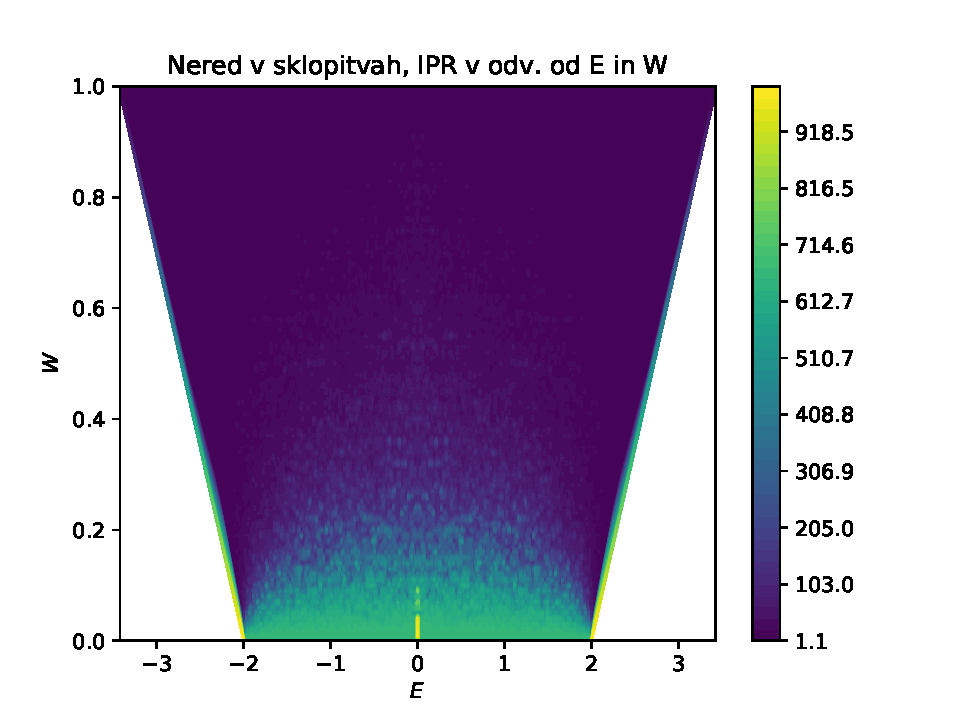
\includegraphics[width=\linewidth]{Figures/SSHIPR2.pdf}
\end{subfigure}
\caption{IPR za primer, ko je nered v sklopitvah. Na $x$ osi je energija stanj, na $y$ pa moč nereda $W$. Za barvo je označen IPR. Graf je izračunan iz verige z dolžino 1000 mest.}
\label{fig:SSHIPR}
\end{figure}

V nadaljevanju bomo obranavali izključno primere, ko imamo nered na sklopitvah brez potencialov na posameznih mestih, torej si poglejmo podrobnejšo teorijo takšnih sistemov.
Obravnavamo Hamiltonjan:
\begin{equation}
\hat{H} = \sum_i g_i | i \rangle \langle i + 1 | + \textup{h. c.},
\end{equation}
kjer so sklopitve $g_i$ neodvisne, enako porazdeljene naključne spremenljivke.
Pokazali bomo, da v tem primeru gostota stanj v okolici energije $E=0$ divergira kot:
\begin{equation}
g(E) \propto \frac{1}{E \log^3 E}
\end{equation}
Schrödingerjeva enačba za zgornji Hamiltonjan se glasi
\begin{equation}
c_{i-1} g_{i-1} + c_{i+1} g_i = E c_i,
\end{equation}
kjer je $c_i$ koeficient lastnega stanja pred vektorjem, lokaliziranem na mestu na verigi $i$.
Vpeljimo količino $\Delta_i = c_{i-1} g_{i-1} / c_i$, ki po Schrödingerjevi enačbi zadošča $\Delta_{i+1} = g_i^2 / (E- \Delta_i)$. Izkaže se \cite{dokazgostota}, da je število stanj do energije $E$ enako deležu pozitivnih $\Delta_i$. Iz rekurzivne formule za $\Delta_i$ vidimo, da pri $E=0$ ti po predznaku alternirajo, kar pomeni, da velja $N(0) = 0.5$.
Poglejmo si $\Delta_i$, ki so pozitivni. Brez izgube splošnosti lahko rečemo, da bodo ti sodi $\Delta_{2i}$.
Iz rekurzivne zveze sledi $\Delta_{2i} = (g_{2i-1}/g_{2i-2})^2 \Delta_{2i-2}$.
Če definiramo $u_{2i} = \ln \Delta_{2i}$, se ta zveza prevede v $u_{2i} = \ln (g_{2i-1}/g_{2i-2})^2 + u_{2i-2}$.
$u_{2i}$ ustrezajo naključnem sprehodu v eni dimenziji, saj velja:
\begin{align}
&\langle u_{2i} - u_{2i-2} \rangle = \langle \ln (g_{2i-1}/g_{2i-2})^2 \rangle = 2 \langle \ln g \rangle - 2 \langle \ln g \rangle = 0 \\
&\langle (u_{2i} - u_{2i-2})^2 \rangle = \langle (\ln (g_{2i-1}/g_{2i-2})^2)^2 \rangle = 2 \langle (\ln g^2)^2 \rangle - 2 \langle \ln g^2 \rangle^2 = 2 \sigma^2 
\end{align}
Vemo, da naključni sprehodi ustrezajo difuzijskim procesom \cite{diffusion}, kjer za difuzijsko konstanto $D$ velja zveza $\sigma^2(t) = 2Dt$. V zgornji enačbi ima indeks $i$ vlogo časa, torej imamo $D=\sigma^2 / 2$. Označimo z $\phi (n, u)$ verjetnostno gostoto za $u_n$, ki mora zadoščati difuzijski enačbi:
\begin{equation}
2 \frac{\partial \phi (n,u)}{\partial n} = \sigma^2 \frac{\partial^2 \phi (n,u)}{\partial u^2}
\end{equation}
Poglejmo si še primer, ko energija $E$ ni nič, vendar vseeno zelo majhna.
Zaradi kiralne simetrije, se lahko omejimo na primer, ko velja $E > 0$.
Rekurzivna enačba za sode člene $\Delta_{2i}$ pri neničelni energiji je
\begin{equation}
\Delta_{2i} = \left(\frac{g_{2i -1}}{g_{2i-2}} \right)^2 \Delta_{2i-2} \frac{1 - E/\Delta_{2i-2}}{1+ (E \Delta_{2i-2} - E^2)/g_{2i-2}^2}
\end{equation}
V primeru, ko velja $E \ll \Delta_{2i-2} \ll g_{2i-2}^2/E$, so popravki k primeru $E=0$ zanemarljivi. Prej definirana spremenljivka $u$ torej opravlja naključni sprehod, dokler velja
$\ln E \ll u \ll \ln (g^2 / E)$, kjer je $g$ tu neka tipična vrednost sklopitve $g_i$, za katero se bo izkazalo, da ni pomembna. 
Ker imamo torej tudi pri neničelnem $E$ naključni sprehod, lahko tudi ta primer opišemo s prejšnjo difuzijsko enačbo. Poglejmo, kaj se zgodi z $u$, ko se približujemo zgornji in spodnji meji $\ln E$ in $\ln (g^2 / E)$, kar nam bo dalo robne pogoje za našo difuzijsko enačbo.
Pri zgornji meji $\Delta_{2i-2} \sim g^2/E$, imenovalec naraste, kar spet zmanjša $\Delta_{2i}$. Za naš naključni sprehod $u$ to pomeni, da imamo
odbijajočo bariero pri $u_{\textup{max}} = \ln (g^2 / E)$.
Pri spodnji meji, ko $\Delta_{2i-2} \sim E$ členi $\Delta_{2i}$ padajo, ko so enkrat pod $E$, pa se zgodi, da velja 
$\Delta_{2i+1} = g_{2i} / (E - \Delta_{2i}) > 0$. Eden izmed lihih členov, ki so do sedaj bili negativni torej spremeni predznak. Od tu naprej se zgodba ponavalja, členi spet alternirajo po predznaku, vendar so zdaj lihi tisti, ki so pozitivni, sodi pa negativni.
Zdaj imamo torej naslednjo sliko razvoja členov $\Delta_i$: Začnemo pri vrednosti $g^2/E$ (ZAKAJ TU ZAČNEMO), nekaj časa padamo (ker smo na začetku pri odbijajoči barieri) in se začnemo naključno sprehajati.
Ko enkrat pridemo približno na vrednost $E$, se absorbiramo. Po tem se cikel ponovi, le da se vloge lihih in sodih zamenjajo.
Lahko vidimo, da potrebujemo dva cikla, da se eden izmed negativnih členov v alternirajoči vrsti pri $E=0$ spremeni v pozitivnega. ZAKAJ DVA A SE NE PO ENEM? Torej če rečemo, da je $\bar{n}$ povprečno število potrebnih mest, preko katerih se konča en cikel, imamo naslednednjo relacijo za število stanj pod $E$:
\begin{equation}
N(E) - N(0) = N(E) - 0.5 = 1/(2n)
\end{equation}
Število $\bar{n}$ lahko dobimo na naslednji način.
Difuzijsko enačbo za $\phi$ opremimo z robnimi pogoji, katere smo izpeljali (bariera pri $u_{\textup{max}}$ in absorbcija pri $u_{\textup{min}}$)
\begin{align}
& \frac{\partial \phi}{\partial u} \vert_{u = u_{\textup{max}}} = 0 \\
& \phi \vert_{u = u_{\textup{min}}} = 0
\end{align}
Z začetnim pogojem $\phi (u, 0) = \delta ( u - u_{\textup{max}} - \epsilon)$.
Difuzijsko enačbo s temi pogoji lahko rešimo s seperacijo spremenljivk.
Ko imamo rešitev lahko izračunamo:
\begin{equation}
P(n) = \int_{u_{\textup{min}}}^{u_{\textup{max}}} \phi(u,n) \textup{d} u,
\end{equation}
ki je verjetnost,da $u$ ostane med $u_{min}$ in $u_{max}$ (torej se ne absorbira) po n korakih.
Povprečno število ciklov je potem:
\begin{equation}
\bar{n} = \int_0^\infty n \left( - \frac{ \textup{d} P}{\textup{d} n} \right) \textup{d} n = \int_0^\infty P(n) \textup{d} n,
\end{equation}
kjer smo pri prvem enačaju uporabili definicijo pričakovane vrednosti v drugem pa integrirali per partes (robni členi so nič, saj seveda velja $P(\infty) = 0$).
Rešitev je $n =  \ln^2(g^2/E^2) / \sigma^2$ torej:
\begin{equation}
N(E) = 0.5 (1 + \sigma^2 / (\ln (g/E)^2)^2
\end{equation}
Kar pomeni, da je gostota stanj
\begin{equation}
g(E) = \frac{\textup{d} N}{\textup{d} E} = \frac{2 \sigma^2}{E} \frac{1}{\ln^3 (g/E)^2} = \frac{2 \sigma^2}{E |\ln E^2|^3},
\end{equation}
kjer smo lahko $g$ izpustili, saj predstavlja le (končno) aditivno konstantno divergirajočem imenovalcu.

\chapter{Model in metode dela}
V našem primeru bomo v sklopitve v neskončno dolgi verigi dali nered. Model, ki ga obravnavamo je malenkost modificiran SSH model in sicer obravnavamo naslednji Hamiltonjan:
\begin{equation}
\hat{H} = \sum_{n \in \mathbb{Z}} t_n \left( \frac{1}{2} \hat{c}_n^\dagger (\sigma_1 + i \sigma_2) \hat{c}_{n+1} + \textup{h.c.} \right) + m_n \hat{c}_n^\dagger \sigma_2 \hat{c}_n.
\end{equation}
Zaradi podobnosti z ostalimi deli na to temo \cite{mondragon}, je notacija v tem razdelku drugačna, kot v prej obdelanem SSH modelu, vendar lahko vseeno vidimo podobnosti: $t_n$ tukaj ustreza sklopitvi med različnimi osnovnimi celicami (prej $w$), medtem, ko sklopitvi v osnovni celici (prej $v$) ustreza $\pm i m_n$. Ta model ni čisto enak kot SSH model, ker je ena izmed sklopitev imaginarna. Z $c_n$ je označen vektor fermionskih operatorjev na obeh podmrežah, torej
$\hat{c}_n = (\hat{c}_{n,A} , \hat{c}_{n,B})^T$.
Model ima kiralno simetrijo, kjer je operator kiralne simetrije enak
\begin{equation}
\hat{S} = \sum_n \hat{c}_n^\dagger \sigma_3 \hat{c}_n
\end{equation}
Nered bomo realizirali s pomočjo dveh naključno porazdeljenih spremenljivk $\omega_n$ in $\omega_n^\prime$. Ti sta neodvisni in porazdeljeni po enakomerni porazdelitvi v intervalu $[ -0.5 , 0.5]$:
\begin{equation}
\omega_n, \omega_n^\prime \sim \mathcal{U}(-0.5,0.5).
\end{equation}
S temi nakjučnimi števili definiramo sklopitve na naslednji način:
\begin{align}
&t_n = 1 + 0.5 W \omega_n \\
&m_n = m + W \omega_n^\prime
\end{align}
Nered je torej centriran okoli vrednosti $1$ oziroma $m$, njegovo jakost pa podaja število $W$.
Če nered ni prisoten imamo kot v SSH modelu na voljo dve fazi: $\nu=1$, če $m \in (-1,1)$ in $\nu=0$ sicer.

Ureditveni parameter v prisotnosti nereda bo še vedno ovojno število, vendar je njen izračun nekoliko bolj zakompliciran.
Spomnimo se, da smo v čistem sistemu imeli na voljo formulo:
\begin{equation}
\nu = \frac{1}{2 \pi i} \int_0^{2 \pi} \frac{\partial \log h(k)}{\partial k} \textup{d}k = \frac{1}{2 \pi i} \int_0^{2 \pi} \frac{\partial h(k)}{\partial k} \frac{1}{h(k)} \textup{d}k,
\end{equation}
kjer je $h(k)$ bila naddiagonalna komponenta Hamiltonjana v recipročnem prostoru. V prisotnosti nereda nimamo več translacijske invariance in torej tudi nimamo več Blochovega teorema / kristalnega valovnega vektorja. Vidimo, da izraz za ovojno število v recipročnem prostoru torej ne bo dober, zato bomo zgornjo formulo zapisali v realnem prostoru.
To storimo z naslednjima substitucijama:
\begin{align}
&\frac{1}{2 \pi} \int_0^{2 \pi}\  \textup{d}k \to \frac{1}{N} \mathrm{Tr}, \\
&\frac{\partial}{\partial k} \to  -i [X, \cdot ]. 
\end{align}
Zgornja substitucija predstavlja le zapis sledi na enoto volumna v drugi bazi, spodnja pa je aplikacija znane formule za transformacijo operatorjev pri delovanju Liejevih grup \cite{georgi}.
Pomisliti moramo še, s čim nadomestiti $h(k)$, ki se pojavi v integrandu. Izkaže se, da je pravilen odgovor izvendiagonalna komponenta celotnega Hamiltonjana v bločnem zapisu. JE TO RES IN ZAKAJ To lahko hitreje dobimo s homotopsko ekvivalentnim Hamiltonjanom (spomnimo se, da homotopije ohranjajo ovojno število) $Q=P_+ - P_-$, kjer sta $P_\pm$ projektorja na pozitivni oziroma negativni del spektra Hamiltonjana $H$. Sedaj se spomnimo, da za nas operator kiralne simetrije $S$ velja $S^\dagger =S $ in $S^2 = \mathbb{I}$, kar pomeni, da so njegove lastne vrednosti enake $\pm 1$, torej ga lahko zapišemo kot $S = S_+ - S_-$, kjer so $S_\pm$ primerni sprektralni projektorji. Ker ima tudi Hamiltonjan $Q$ kiralno simetrijo, ga lahko zapišemo kot
\begin{equation}
Q = S_+ Q S_- + S_- Q S_+ = Q_{+-} + Q_{-+}.
\end{equation} 
Izvendiagonalni blok Hamiltonjana je potem preprosto $Q_{+-}$, njegov inverz pa $Q_{+-}^{-1} = Q_{-+}$.
Sledi, da se formula za ovojno število glasi KAM ZGINE i?:
\begin{equation}
\nu = -\frac{1}{N} \mathrm{Tr} \left(Q_{-+} [X,Q_{+-}] \right).
\end{equation}
Zgornja formula dobro deluje, če računamo ovojno število za končno verigo brez robnih pogojev. Če pa želimo izračunati ovojno število za sistem s periodičnimi robnimi pogoji (kot jo bomo v nadaljevanju), se moramo v zgornji formuli nekako rešiti operatorja $X$, kajti  pri sistemih s takimi robnimi pogoji je operator ta slabo definiran.
V tem primeru namesto substitucije $\partial_k Q_{+-} \ to -i [X, Q_{+-}]$, odvod po $k$ izrazimo s končnimi diferencami \cite{diference}:
\begin{equation}
\partial_k Q_{+-}(k) = \sum_m c_m Q_{+-} (k+m \Delta ), 
\end{equation}
kjer je razmak najmanjša možna diferenca valovnega vektorja enaka $\Delta  = \frac{4 \pi}{N}$, saj ima naš sistem $N/2$ osnovnih celic.
Odvisnosti od $k$ v operatorju $Q_{+-}$ se lahko znebimo, s pomočjo operatorja $e^{i k \hat{x}}$, ki predstavlja translacijo za moment $k$: 
\begin{equation}
Q_{+-}(k+m \Delta ) =e ^{-i m \Delta  x} Q_{+-}(k) e^{i m \Delta  x}
\end{equation}
Kot prej dobimo potem po prehodu v realni prostor formulo:
\begin{equation}
\nu = \frac{1}{N} \mathrm{Tr} (\sum_m c_m Q_{-+} e^{-im \Delta x} Q_{+-} e^{im \Delta x}).
\end{equation}
V zgornji formuli ni več težav z operatorjem $x$, saj kompleksen eksponent poskrbi za periodičnost.
Iz formule za ovojno število brez periodičnih robnih pogojev je razvidno, da je v limiti močnega nereda $W \to \infty$ ovojno število enako nič, saj v tem primeru vezi v osnovni celici dominirajo in je komutator v formuli enak nič ($X$ označuje osnovno celico, ki so v tej limiti med sabo nesklopljene), medtem ko imamo po drugi strani pri $W=0$ in $m \in (-1,1)$ ovojno število enako ena. Vidimo torej, da lahko med topološkimi fazami prehajamo tudi z večanjem jakosti nereda. Tak prehod je prikazan na Sliki \ref{fig:InvariantVsW}, kjer se vidi, da je prehod zelo strm in se zgodi pri $W=4$. Na sliki je tudi oblika energijskih pasov (valenčnega in prevodnega), kjer vidimo, da se ovojno število spremeni šele nekaj časa po tem, ko se energijska reža zapre, kar se zgodi pri $W=3$.
\begin{figure}[H]
\centering
\begin{subfigure}{.7\textwidth}
\includegraphics[width=\linewidth]{Figures/InvariantVsW.png}
\end{subfigure}
\caption{Ovojno število, ko večamo jakost nereda, kjer smo povprečili po $200$ realizacijah disorderja. Opazimo nenadno spremembo pri približno $W=4$, kar je nekaj po zaprtju energijske reže. Vir Slike: \cite{mondragon}}
\label{fig:InvariantVsW}
\end{figure}

Izkaže se, da je točka faznega prehoda povezana z lokalizacijsko dolžino stanja z ničelno energijo. Zaradi Andersonove lokalizacije so namreč stanja v prisotnosti nereda lokalizirana, a pride pri faznem prehodu do tranzicije v delokalizirano stanje pri energiji nič.
To se da videti iz eksplicitne rešitve Schrödingerjeve enačbe pri energiji nič.
Označimo s $\Psi_{n, \alpha}$ vrednost valovne funkcije $\Psi$ na $n$-ti osnovni celici verige, na podmreži $\alpha$, kjer $\alpha=1$ ustreza podmreži A, $\alpha=-1$ pa podmreži B.
Schrödingerjeva enačba se glasi:
\begin{align}
&H \Psi = 0 \\
&t_n \psi_{n-\alpha, \alpha} + i \alpha m_n \Psi_{n, \alpha} = 0
\end{align}
Iz zgornje enačbe lahko rekurzivno izrazimo rešitev:
\begin{equation}
\Psi_{n+\xi_\alpha, \alpha} = i^n \prod_{j=1}^n \left( \frac{t_j}{m_j} \right)^\alpha \Psi_{\xi_\alpha,\alpha},
\end{equation}
kjer $\alpha = \pm 1$ ustreza $\xi_\alpha = 0, 1$.
Za velike $n$ definirajmo $|\Psi_{n+\xi_\alpha, \alpha}| = e^{-n/\Lambda } |\Psi_{\xi_\alpha, \alpha}|$, saj mora valovna funkcija eksponentno padati, če hočemo, da je normalizabilna. Z $\Lambda$ smo označili lokalizacijsko dolžino stanja.
Iz zgornje rekurzivne enačbe dobimo izraz zanjo:
\begin{equation}
\Lambda^{-1} = \mathrm{max}_{\alpha = \pm 1} \left( - \lim_{n \to \infty} \frac{1}{n} \log |\Psi_{n+ \xi_\alpha, \alpha}| / |\Psi_{\xi_\alpha, \alpha}| \right).
\end{equation}
Ker imamo opravka z dvemi različnimi rekurzivnimi enačbami ($\alpha=1$ in $\alpha=-1$), bi lahko za vsako dobili neko lokalizacijsko dolžino. Smiselno je definirati lokalizacijsko dolžino stanja kot manjšo izmed teh dveh, kar pomeni, da v zgornjem izrazu nastopa $\mathrm{max}_{\alpha = \pm 1}$. JE TO PRAVA RAZLAGA? 
Če vstavimo rekurzivni izraz za $\Psi_{n+ \xi_\alpha, \alpha}$ dobimo (maksimum po $\alpha$ izgine, ker različna izbira $\alpha$ samo spremeni predznak $\Lambda^{-1}$, mi pa vzamemo večjo, torej pozitivno):
\begin{equation} \label{empiricnalok}
\Lambda^{-1} = \left| \lim_{n \to \infty} \frac{1}{n} \sum_{j=1}^n ( \log |t_j| - \log |m_j| ) \right| 
\end{equation}
Zgornji izraz bi radi poenostavili. 
To lahko naredimo s pomočjo Birkhoff-Khinchinovega izreka, kjer naključne spremenljivke $t_j$ in $m_j$ razumemo v smislu verjetnostne mere \cite{mera}:
\begin{theorem*}
Naj bo $f$ merljiva funkcija in $E(|f|) < \infty$. Naj bo $T$ ergodična preslikava. Potem velja:
\begin{equation}
\lim_{n \to \infty} \frac{1}{n} \sum_{k=0}^{n-1} f(T^k x) = E(f)
\end{equation}
\end{theorem*}
V našem primeru je $f(x_1,y_1, x_2, y_2, ...) = \log |x_1| - \log |y_1|$, ki je merljiva funkcija, saj je zvezna. Celoten vzorčni prostor je enak $\Omega\times \Omega \times \Omega\times ...$, kjer je $\Omega = [1-0.5 W_1, 1 + 0.5 W_1] \times [m-0.5 W_2, m+0.5 W_2]$ vzorčni prostor za enega izmed parov naključnih števil. Verjetnostna mera je preprosto Lebesgueova mera, normirana na 1 na teh intervalih. Preslikava $T$ nam generira nov par naključnih števil in deluje kot premik koordinat $T (x_1,y_1,x_2,y_2,...) = (x_2,y_2,x_3,y_3,...)$. Ker sta ti porazdeljeni po isti porazdelitvi, preslikava $T$ ohranja mero. Po Kolmogorovem 0-1 zakonu \cite{diffusion} je $T$ tudi ergodična.
Poglejmo si še pričakovano vrednost $|f|$:
\begin{equation}
E(|f|) = \int_{-0.5}^{0.5} \textup{d} \omega \int_{-0.5}^{0.5} \textup{d} \omega^\prime \left| \log | 1 + W_1 \omega | - \log | m + W_2 \omega^\prime | \right|.
\end{equation}
Ker integriramo po končnem intervalu, je morebiten problematičen del le tisti, kjer ima logaritem divergenco, na primer, ko velja $\omega \sim -\frac{1}{W_1}$. Ko primerno razbijemo integral na manjše intervale in se znebimo absolutne vrednosti v integrandu, dobi tak problematičen del obliko $\lim_{\epsilon \to 0} \int_{- \epsilon}^\epsilon \log |x| dx =  2 \lim_{\epsilon \to 0} \int_{0}^\epsilon \log x dx = \lim_{\epsilon \to 0} x (\log x - 1) \rvert_0^\epsilon = 0$. Del blizu divergence torej k intergalu ne prispeva in velja $E(|f|) < \infty$.

Sedaj lahko direktno uporabimo Birkhoffov izrek, da dobimo:
\begin{equation}
\Lambda^{-1} = \left| \int_{-0.5}^{0.5} \textup{d} \omega \int_{-0.5}^{0.5} \textup{d} \omega^\prime ( \log | 1 + W_1 \omega | - \log | m + W_2 \omega^\prime | ) \right|,
\end{equation}
kar se da analitično izračunati. Rezultat je:
\begin{equation} \label{analiticnalok}
\Lambda^{-1} = \left| \log( \frac{|2+W_1|^{1/W_1 + 0.5} |2m - W_2|^{m/W_2 -0.5}}{|2-W_1|^{1/W_1-0.5} |2m + W_2|^{m/W_2 + 0.5}})\right|.
\end{equation}

\begin{figure}[H]
\centering
\begin{subfigure}{.7\textwidth}
\includegraphics[width=\linewidth]{Figures/CriticalSurface.png}
\end{subfigure}
\caption{Na levi je prikazan fazni diagrami modela. Na desni je prikazana še lokalizacijska dolžina stanja z $E=0$ in lahko vidimo, da ta divergira vzdolž faznega prehoda. Prav tako je na desni s črno črto označena pot po kateri bomo pozneje izvedli preklop Hamiltonjana. Izračuni za $\nu$ so narejeni na verigi velikosti $N=2000$ in povprečeni preko $10$ realizacij nereda. Vir Slike: \cite{mondragon}}
\label{fig:CriticalSurface}
\end{figure}

Na Sliki \ref{fig:CriticalSurface} je prikazan fazni diagram našega modela. Kot prej povedano, lahko poleg navadnega prehoda med fazama, ki smo ga videli že v SSH modelu, med fazama preidemo tudi z dovolj močno jakostjo nereda. Zanimali nas bodo preklopi Hamiltonjana čez fazni prehod, kjer bomo povečevali $W$ pri $m=0$ kot je na desnem grafu značeno s črno črto.
Zaenkrat nekaj o tem faznem prehodu že vemo. Če razvijemo enačbo (\ref{analiticnalok}) okoli $W_C=4$, pri $m=0$, vidimo da lokalizacijska dolžina v bližini faznega prehoda skalira kot $\Lambda \sim \frac{1}{|W-W_C| \log |W-W_C|}$. Kritični eksponent $\nu$ za ta prehod je torej enak ena z logaritemskim popravkom.

Oglejmo si obnašanje modela pri parametrih, ki so na poti vzdolž katere bomo izvedli preklop. 
Kot prvi test in občutek za potrebno velikost verige $N$, si poglejmo primerjavo empirične (\ref{empiricnalok}) in analitične (\ref{analiticnalok}) formule za lokalizacijsko dolžino vzdolž te poti za več velikosti sistema.
\begin{figure}[H]
\centering
\begin{subfigure}{.7\textwidth}
\includegraphics[width=\linewidth]{Figures/locLength.pdf}
\end{subfigure}
\caption{Inverz lokalizacijske dolžine pridobljen z empirično formula za več velikosti sistema ($N$ prikazuje število vseh atomov v verigi) in z analitično formulo za neskončno dolgo verigo vzdolž poti $W: 2 \to 6$ pri $m=0$.}
\label{fig:locLength}
\end{figure}
Na Sliki \ref{fig:locLength} vidimo, da za velikosti verige nekaj tisoč atomov ne pridemo še do točnega asimptotskega obnašanja (Poizkusil sem še večje verige in izkaže se, da bi zato rabili verigo daljšo več 100 tisoč atomov), vendar je obnašanje lokalizacijske dolžine pri tako majhnih verigah vseeno kvalitativno zelo podobno obnašanju neskončne verige. Za večje $N$ postane numerika zelo zahtevna, zato bom pri preostanku magisterija obravnaval verigo z $N=1000$. Vse izračune, ki sledijo sem ponovil za dvakrat daljšo verigo, kjer ni bilo opaziti razlike. Poleg tega lahko na sliki opazimo še eno stvar - ko imamo opravka z določeno realizacijo nereda, je število uporabljenih naključnih števil seveda končno (zaradi končne verige) in se divergenca lokalizacijske dolžine (in s tem fazni prehod) ne zgodi točno pri $W=4$ kot narekuje asimptotska formula vendar nekoliko levo ali desno od te točke. Izkaže se, da to ni problem, saj bomo pri eksitacijah rezultate tako ali tako povprečevali po dovolj veliko realizacijah nereda, da lahko privzamemo, da je povprečna točka faznega prehoda res $W=4$.

V naslednjem grafu si bomo pogledali, kako izgledajo energijski nivoji vzdolž poti čez fazni prehod. 
V ta namen napišimo Hamiltonjan v matrični obliki:
\[
H = \begin{bmatrix} 
0 & i m_1 &  &  &  & t_{N/2}\\
-i m_1 & 0 & t_1 &  & &  \\
 & t_1 & 0 & im_2 &  &  \\
 &  & -im_2 & 0& \ddots&  & \\
 &  &  & \ddots & \ddots & im_{N/2}  \\
t_{N/2} & & &  & -i m_{N/2} & 0  
    \end{bmatrix}
\]
kjer smo za Hamiltonjan izbrali periodične robne pogoje, saj se hočemo čim bolj približati neskončni verigi. Energije bomo dobili z diagonalizacijo Hamiltonjana in sicer bom uporabil metodo eigh za diagonalizacijo hermitskih matrik iz Scipyjeve knjižnice za linearno algebro (Python 3).
Iz spektra lahko izračunamo tudi gostoto stanj. Formalno je to vsota Diracovih delta funkcij pri lastnih energijah:
\begin{equation}
g(E) = \sum_{i=1}^N \delta (E_i - E),
\end{equation}
Za potrebe prikaza bom Diracove delte aproksimiral z Lorentzovo krivuljo:
\begin{equation}
\delta (x) = \lim_{\sigma \to 0} \frac{1}{\pi} \frac{\sigma}{\sigma^2 + x^2}
\end{equation}
V mojih izračunih sem vzel vrednost $\sigma=0.01$.
Rezultati, ki jih numerika da, so sledeči:
\begin{figure}[H]
\centering
\begin{subfigure}{\textwidth}
\includegraphics[width=\linewidth]{Figures/Nicegraph.pdf}
\end{subfigure}
\caption{Nekaj najnižjih lastnih energijskih nivojev vzdolž poti $W: 2 \to 6$ pri $m=0$. S črno črtkano črto (desna y os) je narisana lokalizacijska dolžina za to realizacijo nereda. Na spodnjih treh grafih je za različna mesta vzdolž poti prikazana gostota stanj.}
\label{fig:Nicegraph}
\end{figure}

Na Sliki \ref{fig:Nicegraph} vidimo nekaj najnižjih pozitivnih energijskih nivojev vzdolž poti, kjer bomo izvajali preklop. Slika za negativne je enaka, saj je zaradi kiralne simetrije spekter simetričen. Vidimo, da se pri približevanju kritični točki energijska reža res zapre, energijski nivoji pa se podrobneje obnašajo dosti naključno. Po prehodu skozi kritično točko se energijska reža odpira veliko počasneje in je v praksi kar še vedno zaprta. Opazimo, da se energijski nivoji med seboj večkrat sekajo, pogosto pa se zgodijo tudi avoiding crossingi, kot je na primer prikazano na povečanem izseku dela grafa.
Na grafu je prikazana tudi lokalizacijska dolžina stanja z energijo nič in vidimo lahko, da se v točki kjer ta divergira energijski nivoji res najbolj približajo ničli, kar ustreza faznemu prehodu med topološkima fazama. V resnici gredo čisto na nič, vendar smo tu seveda omejeni z numeriko in končnim sistemom. 
Na spodnjih treh grafih je prikazana gostota stanj, pridobljena za tri točke vzdolž poti. Prva ustreza približno $W=2$, kar je še daleč od kritične točke in energijska reža je še odprta, kar vidimo v ničelni gostoti stanj okoli energije nič. Okoli $W=3$ se energijska reža že zapira, kar lahko potrdimo s tem, da je gostota stanj pri $E=0$ že neničelna. V kritični točki se v gostoti stanj pojavi divergenca v energiji $0$. Točno obliko te divergence pravzaprav že poznamo, saj v kritični točki velja, da so sklopitve $t_n$ in $m_n$ porazdeljene po isti porazdelitvi, kar pomeni, da velja formula, izpeljana v prejšnjem poglavju: $g(E) \propto \frac{1}{E \log^3 E}$.
\begin{figure}[H]
\centering
\begin{subfigure}{.7\textwidth}
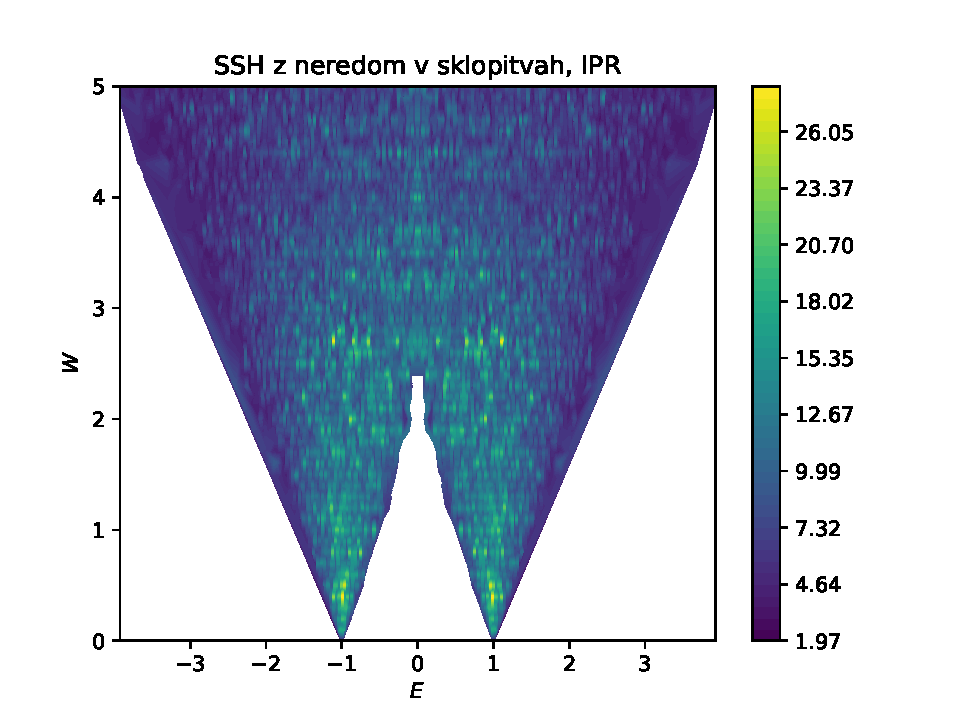
\includegraphics[width=\linewidth]{Figures/SSHIPRNered.pdf}
\end{subfigure}
\caption{Prikaz IPR-ja v odvisnosti od jakosti nereda $W$ in energije $E$ za naš model.}
\label{fig:SSHIPRNered}
\end{figure}
Na Sliki \ref{fig:SSHIPRNered} vidimo IPR za model, ki ga obravnavamo. Tu so že v čistem modelu stanja lokalizirana, saj čisti model tukaj ustreza eni izmed popolnoma dimeriziranih limit v SSH modelu. Ko dodamo nered stanja ostanejo močno lokalizirana. Tudi v okolici točke $W=4, E=0$ ni videti nobene lokalizacije, kar se zdi v nasprotju z našo prejšnjo izpeljavo. Razlog je dejstvo, da delokalizacija velja točno v kritični točki in točno pri energiji nič, kar sta pogoja katerima lahko z numeriko le do neke natančnosti zadostimo in torej tega v praksi ne opazimo zlahka. Na Sliki \ref{fig:EigenPloti} so prikazane verjetnostne gostote nekaterih lastnih funkcij. Vidimo, da so zunaj kritične točke te lokalizirane, v kritični točki pa je tista z najnižjo energijo (približek za energijo nič) delokalizirana. Za prikaz tega obnašanja je bilo treba močno fine-tunati parametre modela, zato tega obnašanja v redkejšem preiskovanju faznega prostora, kot na Sliki \ref{fig:SSHIPRNered} ne bomo našli. NAJBRŽ BOM TU DAL SLIKO IZ ANIMACIJE NA DROPBOXU, KJER SEM VIDEL DA VMES STANJE ZGLEDA DOKAJ DELOKALIZIRANO
\begin{figure}[H]
\centering
\begin{subfigure}{.7\textwidth}
\includegraphics[width=\linewidth]{Figures/EigenPloti.pdf}
\end{subfigure}
\caption{Prve 3 lastne funkcije z pozitivno energijo narisane zunaj in v kritični točki.}
\label{fig:EigenPloti}
\end{figure}

Sedaj se bomo posvetili preklopom Hamiltonjana čez fazni prehod, kar pomeni, da bomo spremljali časovni razvoj valovne funkcije, pri čemer bomo parametre Hamiltonjana linearno spreminjali vzdolž prej omenjene poti.

Preklop bomo delali med dvema vrednostima jakosti nareda, tako da začnemo pri vrednosti $W_{\textup{zac}}<4$, končamo pa, po nekem času preklopa $T$, pri vrednosti $W_{\textup{kon}}>4$.
Časovno odvisnost jakosti nereda lahko torej zapišemo kot 
\begin{equation}
W(t) = W_{\textup{zac}} +  t/T (W_{\textup{konc}}-W_{\textup{zac}}),
\end{equation}
kjer je $T$ dolžina preklopa. 
Začnemo z nekim lastnem stanjem pri $W_{\textup{zac}}$ in ga časovno razvijemo. Ker delamo preklop, je tudi Hamiltonjan odvisen od časa.
Rešujemo torej časovno odvisno Schrödingerjevo enačbo:
\begin{equation}
i \frac{\partial \Psi}{\partial t} = \hat{H}(t) \Psi
\end{equation}
Rešitev izrazimo s pomočjo operatorja časovnega razvoja $\hat{U} = e^{-i \hat{H}}$ kot $\Psi(t) = \hat{U} \Psi(0)$.
Numeričnih metod za izračun časovnega razvoja je več, mi bomo izbrali implicitno metodo tipa Crank-Nicholson, ki zagotavlja, da bo naš operator časovnega razvoja res unitaren.
Uporabili bomo Padéjevo aproksimacijo za eksponentno funkcijo:
\begin{equation}
\exp (-i \tau \hat{H}) = \left(\hat{\mathbb{I}} + i \frac{\tau}{2} \hat{H} \right)^{-1}   \left(\hat{\mathbb{I}} - i \frac{\tau}{2} \hat{H} \right) + \mathcal{O}(\tau^3),
\end{equation} 
s čimer dobimo implicitno shemo:
\begin{equation}
\left( \hat{\mathbb{I}} + i \frac{\tau}{2} \hat{H}(t) \right) \Psi (t+\tau) = \left(\hat{\mathbb{I}}- i \frac{\tau}{2} \hat{H}(t) \right) \Psi(t).
\end{equation}
V našem primeru bomo časovno razvijali več funkcij hkrati. To bi lahko preprosto storili tako, da bi zgornjo enačbo reševali za vsako izmed njih, a je učinkoviteje, če rešujemo samo eno matrično enačbo:
\begin{equation}
\left( \mathbb{I} + i \frac{\tau}{2} \hat{H}(t) \right) X(t+\tau) = \left(\mathbb{I}- i \frac{\tau}{2} \hat{H}(t) \right) X,
\end{equation}
kjer so v matriki $X$ lastni vektorji $\Psi$ v stolpcih.
Za učinkovito reševanje te enačbe, bomo za množenje matrik uporabili Scipyjevo funkcijo za sparse matrike Scipy.sparse, saj imamo opravka s sparse Hamiltonjanom.
V našem primeru bomo vzeli vrednost $\tau=1$. Rezultate smo preverili tudi pri $\tau=0.5$, kjer nismo opazili nobene razlike.

Med preklopom se pojavijo eksitacije v prevodnem pasu, saj je čas preklopa končen.
Število eksitacij v i-to stanje oziroma zasedenost i-tega stanja izračunamo preprosto kot
\begin{equation}
N_i = \sum_j |\langle i | \Psi_j \rangle|^2,
\end{equation}
kjer je $\Psi_j$ časovno razvito j-to stanje iz valenčnega pasu, $| i \rangle$ pa predstavlja i-to lastno stanjo Hamiltonjana ob nekem času. Vrednost $| \langle i | \Psi_j \rangle |^2$ je verjetnost, da elektron iz časovno razvitega stanja j preskoči v stanje i. Celotno verjetnost za prehod v stanje i in s tem zasedenost stanja i potem dobimo tako, da to seštejemo po vseh stanjih iz valenčnega pasu j.

Pri obravnavi eksitacij bomo iskali odvisnosti oblike 
\begin{equation}
N_{\textup{eks}} = \alpha T^{\beta},
\end{equation}
kjer nas bo predvsem zanimala potenca $\beta$. Za natančno pridobitev le-te iz podatkov, zgornjo enačbo najprej logaritmiramo
\begin{equation}
\log N_{\textup{eks}} = \log \alpha + \beta \log T.
\end{equation}
Z definicijami $y=\log N_{\textup{eks}}$ in $x=\log T$, tako dobimo linearno funkcijo $y=\beta x + \log \alpha$, katero lahko hitro prilagajamo podatkom s pomočjo numpy-jeve funkcije polyfit.

\chapter{Rezultati preklapljanja}
Poglejmo, kakšno je število vseh eksitacij po preklopu za več različnih preklopov. Na levem grafu Slike \ref{fig:Skaliranje} se vidi, da število eksitacij pada z dolžino preklopa, kar je smiselno, saj vemo, da adiabatski preklop ustreza neskončno dolgem preklopu in se v njemu ne pojavijo eksitacije, medtem ko se v nenadnem preklopu te pojavijo.
Prav tako opazimo, da imamo več eksitacij, če preklapljamo na večjem intervalu jakosti nereda $[W_{\textup{zac}}, W_{\textup{kon}}]$. Razlog za to je, da pri najmanjšem intervalu jakosti nereda preklopa ne začnemo dovolj globoko v topološki fazi in smo pravzaprav že na meji, kjer se energijska reža zapira, kot bo vidno na Sliki \ref{fig:SkoziCas}. Vidimo lahko tudi, da število eksitacij skalira kot potenčni zakon, kjer je potenca odvisna od intervala jakosti nereda, preko katerega delamo preklop. Potenčno funkcijo sem prilagodil na tri najpočasnejše preklope s pomočjo Scipy-jeve knjižnice za optimizacijo. Kot bo vidno na Sliki \ref{fig:SkoziCas} so hitrejši preklopi prehitri, kar povzroči, da imamo veliko eksitacij že takoj na začetku preklopa, podobno kot če preklapljamo po premajhnem intervalu jakosti nereda.
\begin{figure}[H]
\centering
\begin{subfigure}{.99\textwidth}
\includegraphics[width=\linewidth]{Figures/Skaliranje3Alt.pdf}
\end{subfigure}
\caption{Na levi je prikazano število vseh eksitacij po koncu quencha v odvisnosti od njegovega časa trajanja na desni pa v odvisnosti od njegove hitrosti. S črtkanimi črtami je prikazana nelinearna ekstrapolacija iz treh točk pri največjih časih $T$. Podatki so prikazani za 3 različne izbire začetnih in končnih točk $W_{\textup{zac}}$ in $W_{\textup{kon}}$}
\label{fig:Skaliranje}
\end{figure}
Pravzaprav je smiselneje gledat število eksitacij v odvisnosti od hitrosti preklopa (Namreč, preklop $3.5 \rightarrow 4.5$ pri $T=10000$ je enako hiter kot preklop $2 \rightarrow 6$ pri $T=40000$), kar je prikazano na desnem grafu Slike \label{fig:Skaliranje}. Tu jasneje opazimo, da sta si preklopa na daljšem intervalu veliko bolj podobna v obnašanju v primerjavi s preklopom na krajšem intervalu. 
\begin{figure}[H]
\centering
\begin{subfigure}{.99\textwidth}
\includegraphics[width=\linewidth]{Figures/SkoziCas.pdf}
\end{subfigure}
\caption{Skupno število eksitacij tekom preklopa, prikazano za več različnih intervalov preklopa in njihovih hitrosti.}
\label{fig:SkoziCas}
\end{figure}

Na Sliki \label{fig:SkoziCas} vidimo prej omenjeno hitro naraščanje števila eksitacij že takoj na začetku preklopa pri ozkem intervalu preklopa in pri hitrih preklopih.
Pri daljših intervalih in počasnejših preklopih vidimo, pa je krivulja na začetku ravna, kar pomeni, da smo začeli dovolj globoko, ko je energijska reža še dovolj široka, da eksitacij ni veliko. Podobno kot v energijskih nivojih imamo tudi tu asimetrijo desne in leve strani.
Na Sliki \ref{fig:SkoziCasAlt} smo graf eksitacij skozi čas v x osi reskalirali, s prej dobljenimi eksponenti za potenčno odvisnost števila eksitacij od dolžine preklopa. Opazimo univerzalno obnašanje krivulj pri preklopih na daljših intervalih, razen morda pri zelo hitrih preklopih.
\begin{figure}[H]
\centering
\begin{subfigure}{.99\textwidth}
\includegraphics[width=\linewidth]{Figures/SkoziCasAlt.pdf}
\end{subfigure}
\caption{Skupno število eksitacij tekom preklopa, prikazano za več različnih intervalov preklopa in njihovih hitrosti, kjer je vsak graf v x smeri reskaliran s primerno potenco, pridobljeno iz Slike \ref{fig:Skaliranje}}
\label{fig:SkoziCasAlt}
\end{figure}

Poglejmo si še kje natančneje se pojavijo te eksitacije. Na Sliki \ref{fig:Krajevne} je prikazana krajevna porazdelitev eksitacij tekom preklopa. Vidimo, da se eksitacije pojavljajo postopoma po nekih naključnih osnovnih celicah.
\begin{figure}[H]
\centering
\begin{subfigure}{.99\textwidth}
\includegraphics[width=\linewidth]{Figures/KrajevneEksitacije.pdf}
\end{subfigure}
\caption{Na sliki so histogrami krajevne porazdelitve eksitacij (na $x$ osi je indeks osnovne celice verige z 500 osnovnimi celicami) za štiri čase tekom quencha, ki skupaj traja $T=100$ in poteka na intervalu $W=[3.5,4.5]$. MOGOČE BI LAHKO ZA DRUG INTERVAL/ČAS QUENCHA RAJE TO DAL.. TO JE EDINO KAR SEM MEL}
\label{fig:Krajevne}
\end{figure}

Poglejmo si še porazdelitev eksitacij po lastnih stanjih Hamiltonjana ob nekem fiksnem času. To je prikazano na Sliki \ref{fig:EksTekom} za dve realizaciji nereda. Kot smo že videli, na začetku še nimamo eksitacij, ker je energijska reža še dovolj široka. Nekje pri $W=4$ se eksitacije začenjajo pojavljati in ostanejo še po preklopu. 
Kot bomo videli še pozneje, je ponavadi po faznem prehodu eksitacij na stanje $0.5$. Včasih se sicer pojavijo stanja, v katerih je število eksitacij blizu $1$ a ti primeri so redkejši, zato se bomo osredotočili na prvega, ki je glede na opažanja veliko bolj tipičen.

\begin{figure}[H]
\centering
\begin{subfigure}{.49\textwidth}
\includegraphics[width=\linewidth]{Figures/EksTekom1.pdf}
\end{subfigure}
\begin{subfigure}{.49\textwidth}
\includegraphics[width=\linewidth]{Figures/EksTekom2.pdf}
\end{subfigure}
\caption{Energijski nivoji in eksitacije za dve realizaciji nereda. Eksitacije predstavlja velikost in barva pikic. Hitrost preklopa je $v=0.01$ na intervalu $W \in [3,5]$.}
\label{fig:EksTekom}
\end{figure}

Na Sliki \ref{fig:EksBini} smo interval energij $E \in [10^{-13},10^{-4}]$ razdelili enakomerno v logaritemski skali na 20 delov (binov) in opazovali eksitacije, ki padejo v te bine, povprečene preko $100$ realizacij nereda. Prikazana sta dva grafa za dve različni hitrosti preklopa. Ta grafa služita le kot še nazornejša slika prej omenjenaga dejstva, da imamo po kritični točki prisotnih veliko več eksitacij kot pred njo in da se pri hitrejšem preklopu eksitacije začnejo pojavljati že nekoliko preden se približamo kritični točki.
\begin{figure}[H]
\centering
\begin{subfigure}{.49\textwidth}
\includegraphics[width=\linewidth]{Figures/EksBini1.pdf}
\end{subfigure}
\begin{subfigure}{.49\textwidth}
\includegraphics[width=\linewidth]{Figures/EksBini2.pdf}
\end{subfigure}
\caption{Eksitacije na interval energije tekom preklopa. Interval $E \in [10^{-13},10^{-4}]$ sem razdelil na 20 delov enakomerno v logaritemski skali in narisal povprečno število eksitacij za vsak interval, povprečeno po $100$ realizacijah nereda.}
\label{fig:EksBini}
\end{figure}
Na Sliki \ref{fig:EksBini2} vidimo podobna grafa, vendar tokrat za večji interval energije $E \in [10^{-13},1]$ in v logaritemski skali. Opazimo, da imajo pri počasnejšem preklopu na koncu najvišje eksitacij manjšo energijo, kot pri hitrejšem. Tudi to bi lahko pričakovali, saj že vemo, da imamo tudi nasploh več eksitacij v hitrejših preklopih.
\begin{figure}[H]
\centering
\begin{subfigure}{.49\textwidth}
\includegraphics[width=\linewidth]{Figures/EksBini3.pdf}
\end{subfigure}
\begin{subfigure}{.49\textwidth}
\includegraphics[width=\linewidth]{Figures/EksBini4.pdf}
\end{subfigure}
\caption{Eksitacije na interval energije tekom preklopa. Interval $E \in [10^{-13},1]$ sem razdelil na 50 delov enakomerno v logaritemski skali in narisal povprečno število eksitacij za vsak interval, povprečeno po $100$ realizacijah nereda. Grafa sta tokrat v logaritemski skali.}
\label{fig:EksBini2}
\end{figure}

Na Sliki \ref{fig:Emax} si podrobneje pogledamo kako je z ravnokar omenjenim višanjem energije končnih eksitacij s hitrostjo preklopa. Opazujemo, pri kateri energiji zasedenost stanj pade iz $0.5$ na $0.25$, kar služi kot ocena za robno energijo nad katero ni več veliko eksitacij. Če to narišemo v odvisnosti od hitrosti preklopa opazimo, da je odvisnost spet potenčna in skalira približno korensko.
\begin{figure}[H]
\centering
\begin{subfigure}{.6\textwidth}
\includegraphics[width=\linewidth]{Figures/EmaxP200.pdf}
\end{subfigure}
\caption{Na grafu je prikazana energija najvišje zasedenih stanj po koncu quencha za več hitrosti quencha. To je energija, kjer eksitacije prvič padejo na $0.25$. Rezultati so povprečeni po $100$ realizacijah nereda, uporabljenih pa je $500$ binov.}
\label{fig:Emax}
\end{figure}

Na Sliki \ref{fig:IzEngaStanja} lahko vidimo, kam točno lahko prehaja elektron, ki je na začetku v nekem določenem stanju (tukaj je na sliki prvo stanje z negativno energijo, vendar je slika podobna za ostala nizkoenergijska stanja). Opazimo, da po kritični točki z verjetnostjo približno $0.5$ preidemo v prevodni pas, kjer imamo praviloma na voljo dve stanji v kateri lahko preidemo z nezanemarljivo verjetnostjo in sicer z verjetnostjo $0.5$ v vsako izmed njiju, pogojno na to, da smo v prevodnem pasu. Ti stanji v kateri lahko skočimo sta ravno kiralna partnerja stanj, v katerih ostanemo, če se ne zgodi skok v prevodni pas.  
\begin{figure}[H]
\centering
\begin{subfigure}{\textwidth}
\includegraphics[width=\linewidth]{Figures/IzEngaStanja.pdf}
\end{subfigure}
\caption{Na grafu je z barvo prikazana verjetnost za prehod v različna lastna stanja Hamiltonjana tekom preklopa, če preklapljamo lastno stanje, ki ima na začetku najvišjo negativno energijo (torej prvo stanje v valenčnem pasu) pri neki realizaciji nereda. Zraven je prikazan še zaporedno število stanja, v katera prehajamo.}
\label{fig:IzEngaStanja}
\end{figure}

Opazili smo, da se po prehodu skozi točko faznega prehoda lahko indeksi zasedenih stanj še nadaljno spreminjajo. Razlago za to lahko vidimo na Sliki \ref{fig:IzEngaStanjaWBand}. Po prehodu ostanejo energijski nivoji tesno blizu in se pogosto križajo ali pa se dogajajo avoided crossingi, kar povzroči , da se naše začetno stanje preimenuje v drugega.

\begin{figure}[H]
\centering
\begin{subfigure}{\textwidth}
\includegraphics[width=\linewidth]{Figures/IzEngaStanjaWBand.pdf}
\end{subfigure}
\caption{Na grafu so poleg verjetnosti za prehod v različna lastna stanja v prevodnem pasu prikazani še energijski nivoji tekom preklopa.}
\label{fig:IzEngaStanjaWBand}
\end{figure}
%\input{Zaklju"cek}
\chapter{Zaklju"cek}
Obravnavali smo SSH model z imaginarno sklopitvijo v osnovnih celicah. Model ustreza eno dimenzionalnem topološkem izolatorju z dvema topološkima fazama, katera klasificira ovojno število. V sklopitve smo dodali nered, kar povzroči, da se lastna stanja lokalizirajo. Čeprav sta topološki fazi dokaj robustni na dodatek nereda, lahko vseeno pridemo do faznega prehoda, če je jakost nereda dovolj močna. Na širšem območju okoli točke faznega prehoda je energijske reža zaprta, na točki faznega prehoda pa se pojavi delokalizirano lastno stanje.  
Izvajali smo preklop preko te točke faznega prehoda in opazovali eksitacije v prevodnem pasu, ki se med tem pojavijo. Ugotovili smo, da te univerzalno skalirajo s hitrostjo preklopa potenčno z nenavadnimi potencami. Prav tako smo potenčni zakon opazili pri skaliranju maksimalnih energij, katere eksitacije zavzamejo po koncu preklopa, kjer smo opazili približno korensko odvisnost od hitrosti preklopa.
Videli smo, da v točki faznega prehoda časovno razvito stanje iz valenčnega pasu praviloma preide v dve različni stanji v prevodnem pasu z enako verjetnostjo. Razlaga tega pojava bi lahko bilo dobro izhodišče za nadaljne raziskave preklopov v obravnavanem modelu. Izkaže se, da lahko s pomočjo Jordan-Wignerjeve transformacije naš Hamiltonjan preslikamo na Heisenbergov model, kjer različne topološke faze ustrezajo sklaplanjem različnih spinov v singlete. V točki faznega prehoda se torej pari spinov v singletu zamenjajo, kar bi utegnilo pojasniti prehod iz enega samega stanja v valečnem pasu v dve stanji v prevodnem.

%--------------------------------------------------------------------------------
%       LITERATURA
%--------------------------------------------------------------------------------

\cleardoublepage\phantomsection
\renewcommand\bibname{Literatura}
\addcontentsline{toc}{chapter}{Literatura}
%\begin{thebibliography}{17}
%\bibitem{kibble} A. del Campo and W. H. Zurek, arXiv:1310.1600, 
%\bibitem{SSH} W. P. Su, J. R. Schrieffer, and A. J. Heeger, Physical Review Letters \textbf{42}, 1698 (1979).
%\bibitem{ashcroft} N. D. Mermin and N. W. Ashcroft, \textit{Solid State Physics} (Brooks cole, 1976).
%\bibitem{madzar} J. K. Asbóth, L. Oroszlány, and A. Pályi, \textit{A Short Course on Topological Insulators: Band Structure and Edge States in One and Two Dimensions} (Springer International Publishing, 2016).
%\bibitem{hatcher} A. Hatcher, \textit{Algebraic Topology} (Cambridge University Press, 2001).
%\bibitem{arxiv} N. Batra and G. Sheet, arXiv:1906.08435.
%\bibitem{proof} B.-H. Chen and D.-W. Chiou, Physics Letters A \textbf{384}, 126168 (2020).
%\bibitem{symmetry} J. P. Elliott and P. G. Dawber, \textit{Symmetry in Physics: Volume 1: Principles and Simple Applications} (Macmillan Education UK, 1979).
%\bibitem{yoichi} Y. Ando, Journal of the Physical Society of Japan \textbf{82}, 102001 (2013).
%\bibitem{anderson} C. Guan and X. Guan, \textit{a brief introduction to Anderson Localization} (2019).
%\bibitem{georgi} H. Georgi, \textit{Lie Algebras in Particle Physics} (Addison Wesley Publishing Company, 1982).
%\bibitem{mera} H. R: Pitt \textit{Lectures on Measure Theory and Probability}.
%\bibitem{diffusion} G. R. Grimmett and D. R. Stirzaker, \textit{Probability and Random Processes} (Oxford University Press, 2001).
%\bibitem{randomwalk} J. R. Norris, \textit{Markov Chains} (Cambridge University Press, 1997).
%\bibitem{binomial} L. Yudell, \textit{The Special Functions and Their Approximations} (Academic Press, 1969).
%\bibitem{mondragon} I. M.-Shem, T. L. Hughes, J. Song, and E. Prodan, Physical Review Letters \textbf{113}, 046802 (2014).
%\bibitem{dokazgostota} T. P. Eggarter and R. Riedinger, Physical Review B \textbf{18}, 569 (1978).
%\bibitem{diference} E. Prodan, arXiv:1010.0595.
%\end{thebibliography}
\bibliographystyle{apsrev4-2-fmf-slo}
\bibliography{Bibliografija-slo}

\cleardoublepage
\renewcommand\appendixname{Dodatek}
%\begin{appendices}
%\chapter{Izpeljava Andersonove lokalizacije v 1D}
%TA DEL GRE VERJETNO PROČ
%Obravnavajmo verigo z $N$ členi in označimo z $a_n$ amplitudo valovne funkcije na n-tem mestu.
%Recimo, da imamo v našem modelu potencial $\epsilon_n$ na mestu n, in sklopitev $V_{n, n+1}$ med sosednjima celicama $n$ in $n+1$.
%Schrödingerjeva enačba za tak model se glasi:
%\begin{equation}
%\epsilon_n a_n + V_{n , n+1} a_{n+1} + V_{n-1, n} a_{n-1} = E a_n.
%\end{equation} 
%Če zgornjo enačbo malenkost preoblikujemo, jo lahko zapišemo v naslednji matrični obliki:
%\begin{equation}
%\begin{pmatrix}
%a_{n+1} \\ a_n 
%\end{pmatrix}
%=
%\begin{pmatrix}
%\frac{E-\epsilon_n}{V_{n,n+1}} & \frac{-V_{n-1,n}}{V_{n,n+1}} \\ 1 & 0 
%\end{pmatrix}
%\begin{pmatrix}
%a_{n} \\ a_{n-1} 
%\end{pmatrix}
%= p_n 
%\begin{pmatrix}
%a_{n} \\ a_{n-1} 
%\end{pmatrix}
%\end{equation}
%Definirajmo še A BI MOGU BIT PRODUKT TU OD ENA?
%\begin{equation}
%P_n = \prod_{i=0}^n p_i 
%\end{equation}
%Če s $P_n$ delujemo na vektor $(a_{i+1}, a_i)^T$, dobimo vektor $(a_{n+i+1}, a_{n+i})^T$.
%Če razpišemo matrično množenje $P_n = p_n P_{n-1}$, dobimo rekurzivno formulo za komponente matrike $P_n$ IZ KJE JE TU PRIŠEL SUBSKRIPT n-2. NAPAKA?:
%\begin{align}
%&P_n^{11} = \frac{E-\epsilon_n}{V_{n,n+1}} P_{n-1}^{11} - \frac{V_{n-1,n}}{V_{n,n+1}} P_{n-2}^{11}, \\
%&P_n^{21} = P_{n-1}^{11}, \\
%&P_n^{12} = \frac{E-\epsilon_n}{V_{n,n+1}} P_{n-1}^{12} - \frac{V_{n-1,n}}{V_{n,n+1}} P_{n-2}^{12}, \\
%&P_n^{22} = P_{n-1}^{12}.
%\end{align}
%
%Lokalizacijo bomo pokazali z izračunom upornosti našega materiala. Če upornosti ni, se valovna funkcija lahko prosto propagira po rešetki in je delokalizirana. Če je pa upornost zelo velika, se funkcija ne mora propagirati po rešetki in bo zato lokalizirana.
%
%Za izračun upornosti bomo uporabili formalizem sipalnih matrik. Predstavljamo si, da je naš vzorec z neredom naokoli obdan z istim materialom, vendar brez nereda. Ravni val pošljemo v naš neurejen vzorec materiala z dveh smeri, kot je to razvidno na Sliki \ref{fig:Sipanje}.
%
%\begin{figure}[H]
%\centering
%\begin{subfigure}{\textwidth}
%\includegraphics[width=.5\linewidth]{Figures/Sipanje.pdf}
%\end{subfigure}
%\caption{Z vijolično je označeno območje, ki ustreza verigi z neredom. Zunaj tega območja so valovne funkcije ravni valovi. REFERENCA}
%\label{fig:Sipanje}
%\end{figure}
%
%Sipalna matrika nam da prepustnost $T$ in odbojnost $R$. Upornost materiala je s tema količinama definirana kot
%\begin{equation}
%\rho = R/T
%\end{equation}
%
%Razširimo torej našo domeno na območje zunaj materiala, kjer valovni funkciji ustrezajo ravni vali:
%\begin{align}
%&a_n = A e^{i k d n} + B e^{-i k d n}, \ \ - \infty < n \leq 1, \\
%&a_n = C e^{ikdn} + D e^{- ik d n},  \ \ n \geq N.
%\end{align}
%Z $d$ smo označili razmik med sosednjima mestoma v verigi.
%ZAKAJ TU ZGLEDA, DA SE NA LEVI STRANI RAVNI VAL ZUNAJ MATERIALA RAZTEZA TUDI V NOTRANJOST MATERIALA (n<=1) MEDTEM KO SE NA DESNI STRANI NE? (n >= N)
%
%Definirajmo najprej naslednjo matriko:
%\begin{equation}
%T
%\begin{pmatrix}
%B \\ A
%\end{pmatrix}
%=
%\begin{pmatrix}
%D \\ C
%\end{pmatrix}.
%\end{equation}
%Matrika $T$ nam torej iz amplitud na levi strani materiala da amplitudi na desni strani.
%Po drugi strani nam sipalna matrika $S$ iz amplitud vpadnih valov da amplitude odbitih/prepuščenih valov oziroma:
%\begin{equation}
%S
%\begin{pmatrix}
%A \\ D
%\end{pmatrix}
%=
%\begin{pmatrix}
%B \\ C
%\end{pmatrix}.
%\end{equation}
%Če primerjamo zgornji matrični enačbi vidimo, da lahko komponente matrik $T$ in $S$ med sabo povežemo na naslednji način:
%\begin{align}
%&r = S_{11} = -\frac{T_{12}}{T_{11}}, \\
%&t = S_{21} = \frac{1}{T_{11}},
%\end{align}
%kjer smo uvedli standardne oznake za komponente sipalne matrike $r$ in $t$. Prepustnost in odbojnost se s temi izražata kot
%$T = |t|^2$ in $R = |r|^2$.
%Sledi, da je upornost enaka:
%\begin{equation}
%\rho = \frac{R}{T} = |T_{12}|^2
%\end{equation}
%
%Izračunati moramo torej izvendiagonalno komponento matrike $T$. To bomo storili tako, da jo bomo najprej povezali z prej definirano prehodno matriko $P_N$.
%Valovna funkcija na robu med materialom z neredom in brez njega mora biti zvezna, kar privede do naslednjih enačb ZAKAJ JE TU ROB ŠIROK DVE MESTI IN KAKO SO LAHKO  A0 IN A(N+1) DEL ROBA, ČE JE V MATERIALU SAMO N MEST?:
%\begin{align}
%&a_1 = Ae^{ikd} + Be^{-ikd}, \\
%&a_0 = A+B, \\
%&a_N = C e^{ikdN} + D e^{-ikdN}, \\
%&a_{N+1} = C e^{ikd(N+1)} + De^{-ikd(N+1)}.
%\end{align}
%Prepišimo zgornje enačbe v matrično obliko in dobimo:
%\begin{equation}
%\begin{pmatrix} a_{N+1} \\ a_N \end{pmatrix} = 
%\begin{pmatrix} e^{-ikd} & e^{ikd} \\ 1 & 1 \end{pmatrix} \begin{pmatrix} e^{-ikdN} & 0 \\ 0 & e^{ikdN} \end{pmatrix} \begin{pmatrix} D \\ C \end{pmatrix} =
%\Lambda \theta^{-1} \begin{pmatrix} D \\ C \end{pmatrix}
%\end{equation}
%\begin{equation}
%\begin{pmatrix} a_1  \\ a_0 \end{pmatrix} = \begin{pmatrix} e^{-ikd} &  e^{ikd} \\ 1 & 1 \end{pmatrix} \begin{pmatrix} B \\ A \end{pmatrix} = \Lambda \begin{pmatrix} B \\ A \end{pmatrix}
%\end{equation}
%Če povežemo še vektor $(a_{N+1}, a_N)^T$ z $(a_1, a_0)^T$ s pomočjo prehodne matrike, dobimo izraz za matriko T:
%\begin{equation}
%T =  \theta \Lambda^{-1} P_N \Lambda
%\end{equation} 
%Končno lahko zapišemo izraz za povprečno upornost:
%\begin{equation}
%\langle \rho \rangle = \frac{1}{4} \left( \langle (P_N^{11})^2 \rangle + \langle (P_{N-1}^{11})^2 \rangle +  ( \langle (P_N^{12})^2 \rangle + ( \langle (P_{N-1}^{12})^2 \rangle \right) - \frac{1}{2},
%\end{equation}
%kjer $\langle \rangle$ predstavlja povprečenje preko nereda.
%Iz rekurzivnih formul za komponente prehodne matrike lahko dobimo:
%\begin{equation}
%\begin{pmatrix}  \langle (P_N^{11})^2 \rangle \\ \langle (P_{N-1}^{11})^2 \rangle \end{pmatrix} = R \begin{pmatrix}  \langle (P_{N-1}^{11})^2 \rangle \\  \langle (P_{N-2}^{11})^2 \rangle \end{pmatrix}
%\end{equation}
%\begin{equation}
%\begin{pmatrix} \langle (P_N^{12})^2 \rangle \\ \langle (P_{N-1}^{12})^2 \rangle \end{pmatrix} = R \begin{pmatrix}  \langle (P_{N-1}^{12})^2 \rangle \\  \langle (P_{N-2}^{12})^2 \rangle \end{pmatrix},
%\end{equation}
%kjer je
%\begin{equation}
%R = \begin{pmatrix} \langle \epsilon^2 \rangle \langle V^{-2} \rangle & \langle V^2 \rangle \langle V^{-2} \rangle \\ 1 & 0 \end{pmatrix}.
%\end{equation}
%Matriko $R$ lahko brez težav diagonaliziramo V ČLANKU PRVI ČLEN V KORNEU NI NA KVADRAT?:
%\begin{equation}
%\lambda_\pm = \frac{1}{2} \langle \epsilon^2 \rangle \langle V^{-2} \rangle \pm \sqrt{(\frac{1}{2} \langle \epsilon^2 \rangle \langle V^{-2} \rangle)^2 + \langle V^2 \rangle \langle V^{-2} \rangle}
%\end{equation}
%Cauchy-Schwartzeva  neenakost nam da:
%\begin{equation}
%\langle V^2 \rangle \langle V^{-2} \rangle \geq \langle V^2 / V^2 \rangle = 1,
%\end{equation} 
%kar pomeni, da velja ZAKAJ JE POMEMBNO, DA JE DRUGA LASTNA VREDNOST MANJŠA
%\begin{equation}
%\lambda_+ > 1
%\end{equation}
%in torej upornost skallira na naslednji način: 
%\begin{equation}
%\langle \rho \rangle \propto \lambda_+^N = e^{N \ln \lambda_+}.
%\end{equation}
%Ker je $\ln \lambda_+ > 1$, dobimo eksponento rast upornosti z velikostjo verige ne glede na jakost nereda. Tako je Andersonova lokalizacija v 1D dokazana.
%\chapter{Splošna formula za ovojno število}
%TUKAJ BOM IZPELJAL TISTO FORMULO ZA WINDING NUMBER IN MALO OMENIL KAKŠNE SO TEŽAVE Z NUMERIKO (DA JE OPERATOR X ZA PBC SLABO DEFINIRAN ETC.).
%
%\end{appendices}
%-------------------------------------------------------------------------------------
%       KAZALO (NEOBVEZNO)
%-------------------------------------------------------------------------------------

\cleardoublepage
\printindex

\end{document}